\documentclass[11pt]{article}

\usepackage[utf8]{inputenc}
\usepackage[T1]{fontenc}
\usepackage{amsmath,amssymb}
\usepackage{mathtools}
\usepackage{booktabs}
\usepackage{longtable}
\usepackage{array}
\usepackage[margin=1in]{geometry}
\usepackage{siunitx}
\usepackage{graphicx}
\usepackage[hidelinks]{hyperref}
\usepackage{xcolor}
\usepackage{enumitem}
\usepackage{amsfonts}
\usepackage{textcomp}
\usepackage{tikz}
\usepackage{tcolorbox}
\tcbuselibrary{skins,breakable}
\usetikzlibrary{arrows.meta,positioning,calc}

% Worked-example boxes, for the teaching sections.
\newtcolorbox{worked}[1][]{breakable, enhanced, colback=black!3,
  colframe=black!55, boxrule=0.5pt, left=6pt, right=6pt, top=5pt, bottom=5pt,
  fonttitle=\bfseries, title={#1}}

% siunitx v2 spellings used by some model sections
\providecommand{\celsius}{\degreeCelsius}
\ProvideDocumentCommand\squared{}{\tothe{2}}
\ProvideDocumentCommand\cubed{}{\tothe{3}}

\sisetup{per-mode=symbol}

% ---------- macros, matching the companion model report ----------
\newcommand{\md}{\ensuremath{\dot m}}
\newcommand{\mdw}{\ensuremath{\dot m_{w}}}
\newcommand{\UA}{\ensuremath{U\!A}}
\newcommand{\degC}{\ensuremath{^{\circ}\mathrm{C}}}
% ---------- THUMS-specific ----------
\newcommand{\Ui}{\ensuremath{U_{i}}}
\newcommand{\hm}{\ensuremath{h_{m}}}
\newcommand{\Tm}{\ensuremath{T_{m}}}
\newcommand{\Tre}{\ensuremath{T_{r_{e}}}}
\newcommand{\km}{\ensuremath{k_{m}}}
\newcommand{\rhom}{\ensuremath{\rho_{m}}}
\newcommand{\Amelt}{\ensuremath{A_{\mathrm{melt}}}}
\newcommand{\Vmelt}{\ensuremath{V_{\mathrm{melt}}}}
\newcommand{\Nwells}{\ensuremath{N_{\mathrm{wells}}}}
\newcommand{\etao}{\ensuremath{\eta_{o}}}
\newcommand{\etaf}{\ensuremath{\eta_{f}}}
\newcommand{\code}[1]{\texttt{\small #1}}

\title{\textbf{P2H2P PCM Wellbore Storage}\\[4pt]
\large Mathematical Model of Power-to-Heat-to-Power Conversion\\
with Phase-Change Material in Repurposed Wells\\[6pt]
\normalsize Thermodynamic Cycles, Borehole Resistance Network,\\
Melt-Front Formulations, Sizing and Performance Indices\\[4pt]
\normalsize Model version 0.4a \textperiodcentered\ last updated 2026-09-10 BRT}
\author{Craft \& Hawkins Department of Petroleum Engineering\\
Louisiana State University}
\date{\today}

\begin{document}
\maketitle

\begin{abstract}
This document states the governing equations of THUMS --- thermal storage in
repurposed wells with phase-change material --- as the code actually implements
them. It is a companion to the master-architecture report of the DBHE plant and
follows the same convention: the model is written \emph{against the source
rather than from memory}, and every equation carries the function that evaluates
it.

That convention matters more here than usual. Until this document, the THUMS
equations existed nowhere except as Python. Four Colab notebooks and a
conference paper were produced without a written model statement, and the
principal defect corrected in v0.2 --- the fluid side giving up heat through a
finned surface of \SI{0.4924}{\meter} while the melt front absorbed it through a
bare cylinder of \SI{0.1324}{\meter} --- is of exactly the kind that a document
placing both surfaces on the same page would have exposed immediately.

Section~\ref{sec:overview} fixes notation and states the modelling hypotheses.
Sections~\ref{sec:cycles}--\ref{sec:hydraulics} give the model proper.
Section~\ref{sec:defects} is not an appendix of caveats but part of the
specification: it lists the assumptions that are known to be violated, the two
places where the same physical quantity is given two different formulas, and the
terms that are absent altogether. A reader reproducing these results needs that
section as much as the equations.

Two melt-front formulations are given. Section~\ref{sec:front:legacy} states the
closed-form Stefan solve used through v0.1 and the conference paper;
Section~\ref{sec:front:marched} states the energy-balance formulation that
replaced it. Both remain in the code and are selected by \code{Case.front}, so
the difference between them is measurable rather than arguable.

\medskip
\noindent\textbf{Changes in version 0.3.} Two corrections, both now the default.
The tube-wall and fin conductivity used during charging was corrected from the
PCM liquid value to steel (\S\ref{sec:defects:kw}); and the fin metal is now
excluded from the melted PCM cross-section (\S\ref{sec:front:finmetal}).

\medskip
\noindent\textbf{Changes in version 0.4.} The melt front now carries
\emph{enthalpy} rather than melted area (\S\ref{sec:front:enthalpy}), so the PCM
may superheat above $\Tm$ once fully molten and subcool below it once fully
solid. Formulation~B previously had nowhere to put heat delivered to a saturated
segment and discarded it --- on discharge the discarded heat reached
\SI{148}{\percent} of the heat delivered. Three things follow: no heat is
clipped, the local melt fraction is confined to $[0,1]$ by construction, and
desuperheating and subcooling are recovered during discharge. The well count is
now set by a \emph{capacity} criterion (\S\ref{sec:hydraulics:capacity}) rather
than by the melted-volume constraint of v0.3.

The consequence worth noting is not the headline number but the
\emph{uniformity}: sensible heat is self-levelling, because a segment that
finishes melting superheats, its driving temperature difference collapses, and
the heat passes downstream. The spread in local melt fraction along the well
falls from $1.321$ to $0.078$.

\medskip
\noindent\textbf{Changes in version 0.4a.} No physics. Two reporting
corrections, both of which changed a conclusion.
Section~\ref{sec:front:enthalpy} is rewritten at length as a teaching treatment
of Formulation~C --- the choice of state variable, the enthalpy curve, the
branchwise-exact integration and its verification, and the failures that
motivated each.
Section~\ref{sec:hydraulics:capacity} adds a reporting rule:
$N_{\mathrm{capacity}}$ is a lower bound and must not be read across a parameter
sweep on its own, because $\Nwells$ is a maximum and the binding criterion
changes.
Section~\ref{sec:defects:h3} corrects the geometric limit on the melt front from
the borehole wall to the \emph{cell} radius, Eq.~\eqref{eq:rcell} --- the old
check was a factor $2.9$ too permissive in $\delta$ and could never fire. Under
Formulation~C the corrected limit cannot be violated, but it is being
\emph{saturated} over \SI{99}{\percent} of the well, which now bears on the fin
count and is the leading open item.
Section~\ref{sec:front:segeq} derives the segment equation in full --- the two
control volumes, the quasi-steady fluid approximation and what it costs, and why
the closing conductance is $\md c_{p}(1-e^{-\mathrm{NTU}})/\Delta z$ rather
than $\Ui P_{i}$, a difference reaching \SI{33}{\percent} here.
A ninth hypothesis, \textbf{H9}, is stated explicitly for the first time:
perfect azimuthal insulation between the cascade layers of a hairpin's two legs,
which at the wellhead are \SI{48.9}{\kelvin} apart. It is assumed perfect for
now and quantified in \S\ref{sec:defects:h9}, where the neglected leak is of
order \SI{25}{\percent} of the useful duty.
\end{abstract}

\tableofcontents
\clearpage

%=====================================================================
\section{Scope, hypotheses and notation}
\label{sec:overview}

THUMS stores electrical energy as latent heat in a phase-change material packed
into the annulus of a repurposed oil-and-gas well. A high-temperature heat pump
melts the PCM during charging; an organic Rankine cycle recovers the energy
during discharging. The storage medium is a trimodal PCM melting at
\SI{150}{\celsius}; the heat-transfer fluid is pressurised water; the borehole
contains longitudinally finned hairpin tubes.

The model answers two questions: \emph{how many wells does a given power block
need}, and \emph{what round-trip efficiency does the resulting plant achieve}.
Everything below serves those two numbers.

%---------------------------------------------------------------------
\subsection*{Headline results, version 0.4}

\begin{center}
\begin{tabular}{@{}l r r r@{}}
\toprule
 & v0.1 published & marched, old $k_{w}$ & \textbf{v0.4} \\
\midrule
$\Nwells$                     & 24.123 & 22.431 & \textbf{11.573} \\
binding constraint            & --- & charge rate & \textbf{capacity} \\
$\varepsilon_{\mathrm{PCM}}$  & 0.5200 & 0.5402 & \textbf{0.9992} \\
local $\varepsilon$, min--max & --- & 0.46--1.78 & \textbf{0.922--1.000} \\
$\eta_{\mathrm{RTE}}$         & 0.43027 & 0.42955 & 0.41585 \\
$\eta_{\mathrm{RTE}}^{0}$     & 0.43484 & 0.43484 & 0.43484 \\
$\mathrm{COP}$                & 2.95633 & 2.95633 & 2.95633 \\
$\eta_{\mathrm{ORC}}$         & 0.23685 & 0.23685 & 0.23685 \\
$\eta_{\mathrm{storage}}$     & --- & 0.953 & 0.9364 \\
closure error                 & 3--54\,\% & $10^{-16}$ & $10^{-16}$ \\
\bottomrule
\end{tabular}
\end{center}

\noindent The sizing moves a long way and the efficiency hardly at all:
$\Nwells$ falls by \SI{52}{\percent} while $\eta_{\mathrm{RTE}}$ moves by about
\SI{3}{\percent}. $\eta_{\mathrm{RTE}}^{0}$ is identical to twelve significant
figures throughout --- the cycles are untouched by any of this. What the storage
model determines is how much hardware the cycle needs, not how efficiently it
runs.

%---------------------------------------------------------------------
\subsection{The structure of the model}

The calculation is a chain, not a coupled system. Each stage consumes the
previous stage's output and nothing flows backwards:

\begin{enumerate}[itemsep=1pt]
\item the ORC and heat-pump cycles fix $\eta_{\mathrm{ORC}}$ and
      $\mathrm{COP}$ from CoolProp property calls alone
      (\S\ref{sec:cycles:states});
\item an energy budget converts the specified electrical output into a charging
      heat duty and a secondary-fluid mass flow (\S\ref{sec:cycles:budget});
\item a resistance network gives the local overall coefficient $\Ui$ along the
      tube (\S\ref{sec:network});
\item an effectiveness--NTU march integrates the fluid temperature down the
      tube, segment by segment (\S\ref{sec:front:march});
\item a melt-front model converts the delivered heat into a melted volume
      (\S\ref{sec:front:legacy} or \S\ref{sec:front:marched});
\item the well count is chosen so that the field satisfies its constraints, and
      the performance indices follow (\S\ref{sec:hydraulics}).
\end{enumerate}

The consequence worth stating explicitly is that the cycles are decoupled from
the storage. $\eta_{\mathrm{ORC}}$ and $\mathrm{COP}$ do not depend on anything
the borehole does. No change to the storage model can move them, which is why
the ideal round-trip efficiency $\eta_{\mathrm{RTE}}^{0}$ of
Eq.~\eqref{eq:rte0} is invariant across every formulation in this document.

%---------------------------------------------------------------------
\subsection{Modelling hypotheses}
\label{sec:overview:hypotheses}

The following are assumed throughout. Those known to be violated in the
operating regime are revisited in \S\ref{sec:defects}.

\begin{description}[leftmargin=1.6em,itemsep=2pt]
\item[H1 --- Quasi-steady conduction.] The melt layer carries no thermal mass.
  Its temperature profile is the steady cylindrical profile corresponding to the
  instantaneous front position. Time enters the model \emph{only} through the
  front position. The hypothesis is controlled by the Stefan number
  \begin{equation}
    \mathrm{Ste} \;=\; \frac{c_{p,m}\,\Delta T}{\hm},
    \label{eq:stefan-number}
  \end{equation}
  and degrades as it grows; at the design point $\mathrm{Ste}=0.0474$.
\item[H2 --- No axial conduction.] Neither the tube wall nor the PCM conducts
  along the well. Segments are coupled only through the fluid stream. This one
  is safe by a wide margin: the axial diffusion time over a segment is
  $\Delta z^{2}/\alpha_{l}=\SI{5.4e9}{\second}$ against a
  \SI{3.6e4}{\second} window (\S\ref{sec:front:segeq}).
\item[H3 --- Concentric annular front.] The melt region around each tube is a
  cylindrical annulus of uniform thickness $\delta$, so that the melted
  cross-section is $\pi[(r_e+\delta)^2-r_e^2]$. Fronts from neighbouring tubes
  do not interact and do not merge. \emph{Under Formulation~C this cannot be
  violated, but it is saturated over the whole well --- see
  \S\ref{sec:defects:h3}.}
\item[H4 --- Conduction only in the melt.] No natural convection in the liquid
  PCM. This is conservative early and increasingly wrong as $\delta$ grows.
\item[H5 --- Enthalpy state, no radial resolution.] \emph{Revised in v0.4.} The
  PCM carries latent \emph{and} sensible energy, lumped into one enthalpy per
  segment (\S\ref{sec:front:enthalpy}): fully molten PCM superheats, fully solid
  PCM subcools. What is still absent is any radial resolution of temperature
  \emph{within} a phase --- each segment has a single PCM temperature, so the
  thermal gradient through the melt layer is quasi-steady (H1) rather than
  resolved.
\item[H6 --- Adiabatic borehole wall.] No heat exchange with the formation in
  either direction, and no geothermal gradient in the energy balance.
\item[H7 --- Incompressible, single-phase secondary fluid.] Pressurised water at
  constant $P$; no buoyancy head in the vertical loop. The fluid is also taken
  as \emph{quasi-steady}: $\partial T/\partial t$ is dropped from its energy
  equation, which costs an unresolved startup transient of about
  \SI{38}{\minute} in each half-cycle (\S\ref{sec:front:segeq}).
\item[H8 --- Multilayer PCM.] The well is divided into $N_{\mathrm{lay}}$ axial
  layers of distinct melting temperature, so that the PCM melting point follows
  the fluid glide down the well. Layer boundaries are equally spaced along the
  \emph{developed} tube length $L_{\mathrm{tube}}$, not the depth --- so a
  hairpin's down leg and return leg belong to \emph{different} layers at the
  same depth. See H9.
\item[H9 --- Perfect azimuthal insulation.] \emph{New in v0.4a, and the
  weakest assumption in the set.} Each tube leg owns an equivalent PCM cell of
  radius $r_{\mathrm{cell}}$ (Eq.~\eqref{eq:rcell}) whose outer boundary is
  adiabatic: no heat crosses between the cells of neighbouring legs at the same
  depth. Because H8 cascades along the developed length, those neighbours are at
  \emph{different} melting temperatures --- up to \SI{48.9}{\kelvin} apart at
  the wellhead, falling to zero at the well bottom where the two legs meet. The
  assumption therefore requires a physical partition between the down-leg and
  return-leg PCM \emph{and} that the partition be insulating. Neither is
  designed, costed, or modelled. A slab estimate puts the neglected leak at
  $\sim\SI{22}{\watt\per\meter}$ against a useful duty of
  $\sim\SI{83}{\watt\per\meter}$ at the wellhead --- of order
  \SI{25}{\percent}, and acting to erase precisely the temperature separation
  the cascade exists to create. Held as an idealisation pending evaluation;
  \S\ref{sec:defects:h9}.
\end{description}

%---------------------------------------------------------------------
\subsection{Geometry}
\label{sec:overview:geometry}

One borehole of diameter $D_{\mathrm{well}}$ and depth $L_{\mathrm{well}}$
contains $n_{t}$ hairpin tubes. A hairpin runs down and back, so its developed
length is
\begin{equation}
  L_{\mathrm{tube}} \;=\; 2\,L_{\mathrm{well}},
  \label{eq:Ltube}
\end{equation}
and the number of tube \emph{legs} in the borehole is $2n_{t}$. This
factor-of-two bookkeeping is a recurring source of error: per-borehole
quantities multiply the per-tube result by $n_{t}$, not by $2n_{t}$, because
Eq.~\eqref{eq:Ltube} has already counted both legs.

The distinction between the developed coordinate $s\in[0,L_{\mathrm{tube}}]$
and the depth $d$ matters wherever a profile is plotted or a layer assigned:
\begin{equation}
  d(s) =
  \begin{cases}
    s, & s \le L_{\mathrm{well}} \quad\text{(down leg)},\\
    L_{\mathrm{tube}} - s, & s > L_{\mathrm{well}} \quad\text{(return leg)}.
  \end{cases}
  \label{eq:depth-fold}
\end{equation}
Every depth therefore carries \emph{two} legs of the same hairpin, at developed
positions $s$ and $L_{\mathrm{tube}}-s$, and by H8 those two are in different
PCM layers. H9 assumes they do not exchange heat.

Each leg carries $n_{f}$ longitudinal fins of thickness $t_{f}$ and radial
length $L_{f}$. The PCM volume available in one borehole is the borehole volume
less the tubes and their fins,
\begin{equation}
  V_{\mathrm{well}}
  \;=\;
  \frac{\pi D_{\mathrm{well}}^{2}}{4}\,L_{\mathrm{well}}
  \;-\;
  2n_{t}\Bigl(\pi r_{e}^{2} + n_{f} t_{f} L_{f}\Bigr) L_{\mathrm{well}} .
  \label{eq:Vwell}
\end{equation}

Equation~\eqref{eq:Vwell} deserves a second look, because it is the source of a
reporting trap taken up in \S\ref{sec:hydraulics:capacity}: fin metal displaces
PCM, so \emph{any} change to the fins moves $V_{\mathrm{well}}$ and hence the
storage capacity of a borehole, entirely independently of what the fins do
thermally.

\emph{Source:} \code{thums\_core/config.py}, class \code{Geometry}.

%---------------------------------------------------------------------
\subsection{Nomenclature}

\begin{longtable}{@{}l l l@{}}
\toprule
symbol & meaning & unit \\
\midrule
\endhead
$\Amelt$ & melted cross-section per unit tube length & \si{\meter\squared} \\
$A_{\mathrm{flow}}$ & tube flow area, $\pi r_{i}^{2}$ & \si{\meter\squared} \\
$d$ & depth below surface & \si{\meter} \\
$s$ & developed tube coordinate & \si{\meter} \\
$A_{\mathrm{avail}}$ & PCM cross-section owned by one segment & \si{\meter\squared} \\
$C_{s}$, $C_{l}$ & sensible capacity per unit tube length & \si{\joule\per\meter\per\kelvin} \\
$E'$ & PCM enthalpy per unit tube length & \si{\joule\per\meter} \\
$E'_{\mathrm{lat}}$ & latent capacity per unit tube length & \si{\joule\per\meter} \\
$K$ & segment conductance per unit tube length & \si{\watt\per\meter\per\kelvin} \\
$c_{p}$ & specific heat capacity & \si{\joule\per\kilogram\per\kelvin} \\
$D_{\mathrm{well}}$ & borehole diameter & \si{\meter} \\
$\hm$ & latent heat of fusion & \si{\joule\per\kilogram} \\
$h_{i}$ & internal convective coefficient & \si{\watt\per\meter\squared\per\kelvin} \\
$h_{e}$ & melt-layer conductance, outer side & \si{\watt\per\meter\squared\per\kelvin} \\
$\km$ & PCM thermal conductivity & \si{\watt\per\meter\per\kelvin} \\
$k_{w}$ & tube-wall and fin conductivity & \si{\watt\per\meter\per\kelvin} \\
$L_{f}$, $t_{f}$, $n_{f}$ & fin length, thickness, count & \si{\meter}, \si{\meter}, -- \\
$L_{\mathrm{well}}$, $L_{\mathrm{tube}}$ & well depth, developed tube length & \si{\meter} \\
$\md$ & mass flow rate & \si{\kilogram\per\second} \\
$n_{t}$ & hairpin tubes per borehole & -- \\
$N_{\mathrm{lay}}$ & PCM layers along the well & -- \\
$\Nwells$ & number of boreholes & -- \\
$\mathrm{NTU}$ & number of transfer units, per segment & -- \\
$q'$ & heat rate per unit tube length & \si{\watt\per\meter} \\
$r_{i}$, $r_{e}$ & tube inner and outer radius & \si{\meter} \\
$r_{\mathrm{cell}}$ & equivalent cell radius of one tube leg & \si{\meter} \\
$R'$ & thermal resistance referred to inner area & \si{\meter\squared\kelvin\per\watt} \\
$R''_{f,i}$ & internal fouling resistance & \si{\meter\squared\kelvin\per\watt} \\
$t_{\mathrm{ch}}$, $t_{\mathrm{dc}}$ & charging, discharging duration & \si{\hour} \\
$\Tm$ & PCM melting temperature & \si{\kelvin} \\
$T_{\mathrm{pcm}}$ & PCM temperature, recovered from $E'$ & \si{\kelvin} \\
$\Tre$ & tube outer-surface temperature & \si{\kelvin} \\
$\Ui$ & overall coefficient on inner area & \si{\watt\per\meter\squared\per\kelvin} \\
$V_{\mathrm{well}}$, $\Vmelt$ & PCM volume, melted volume & \si{\meter\cubed} \\
$\delta$ & melt-layer thickness & \si{\meter} \\
$\delta_{\mathrm{merge}}$ & thickness at which neighbouring fronts touch & \si{\meter} \\
$\Delta z$ & segment length & \si{\meter} \\
$\varepsilon_{\mathrm{PCM}}$ & melted fraction of the PCM inventory & -- \\
$\varepsilon_{\mathrm{local}}$ & melted fraction of one segment's PCM & -- \\
$\etaf$, $\etao$ & fin and overall surface efficiency & -- \\
$\lambda$ & assumed storage-loss surplus & -- \\
$\rhom$ & PCM density & \si{\kilogram\per\meter\cubed} \\
\bottomrule
\end{longtable}

Subscripts $s$ and $l$ denote the solid and liquid PCM phases. Subscripts
$\mathrm{ch}$ and $\mathrm{dc}$ denote charging and discharging. A prime on a
resistance denotes referral to the inner tube area, and a prime on a heat rate
denotes per unit tube length.

%=====================================================================
\section{Thermodynamic cycles and the energy budget}
\label{sec:cycles}

%---------------------------------------------------------------------
\subsection{State points}
\label{sec:cycles:states}

The plant contains two cycles. During charging a two-stage high-temperature heat
pump with two regenerators lifts heat from a source at $T_{\mathrm{source}}$ to
the PCM melting temperature. During discharging a two-stage organic Rankine
cycle rejects to a sink at $T_{\mathrm{sink}}$. Both use cyclopentane; the
secondary fluid circulating through the boreholes is pressurised water.

Every state point is fixed by a specified approach temperature rather than by a
component model. Writing $\Tm$ for the PCM melting point,
\begin{align}
  T_{1e} &= T_{\mathrm{sink}} + \Delta T_{\mathrm{sink,glide}}
            + \Delta T_{E,\mathrm{sink}}, &
  T_{3d} &= \Tm^{\mathrm{bot}} - \Delta T_{M,1D}, \\
  T_{2d} &= T_{3d} + \Delta T_{3D,2D}\ \text{(provisional)}, &
  T_{3e} &= \min\!\left(T_{2d}-\Delta T_{2D,3E},\,
                        T_{3e}^{\mathrm{pinch}}\right), \\
  T_{4c} &= \Tm + \Delta T_{4C,M}, &
  T_{4a} &= T_{\mathrm{source}} - \Delta T_{3A,4A}, \\
  T_{13h} &= T_{4a} - \Delta T_{\mathrm{pinch,HPE}}, &
  T_{3c} &= T_{4c}, \\
  T_{2c} &= T_{3c} - \Delta T_{3C,2C}, &
  T_{2h} &= T_{3c} + \Delta T_{2H,3C},
\end{align}
with
\begin{equation}
  \Tm^{\mathrm{bot}} \;=\; \Tm - \Delta T_{\mathrm{cascade}}\,
  \frac{N_{\mathrm{lay}}-1}{N_{\mathrm{lay}}}
  \label{eq:Tmbot}
\end{equation}
the melting temperature of the coldest cascade layer, \SI{101.111}{\celsius} for
the default case. Function: \code{T\_m\_bottom}, \code{cycle\_state\_points}.

Three of these approaches are \emph{derived} rather than free, and saying so is
the point of the arrangement above. $T_{13h}$ follows from the source outlet
(\S\ref{sec:defects:hpe}); $T_{3e}$ is the smaller of two constraints
(\S\ref{sec:cycles:pinch}); and $T_{1e}$ is referenced to the sink
\emph{outlet}, which coincides with its inlet only because
$\Delta T_{\mathrm{sink,glide}}=0$ models the sink as a reservoir.

The charging glide $\Delta T_{3C,2C}$ is the principal design variable of the
study, and since v0.6 its only job is to set the two mass flow rates. Until
v0.9b the discharging glide and the cascade grading were not separate fields at
all: both were $\Delta T_{3C,2C}$. They are now
$\Delta T_{3D,2D}$ and $\Delta T_{\mathrm{cascade}}$, each defaulting to it, and
\S\ref{sec:cycles:glides} sets out which of the resulting equalities are forced
by energy conservation and which were merely assumed.

\subsection{Which temperatures may be prescribed}
\label{sec:cycles:closure}

The arrangement above changed in v0.6, and the reason is worth stating because
it is easy to get wrong in either direction.

\emph{Only the two exchanger inlets are boundary conditions.} $T_{4c}$ and
$T_{3d}$ are what the marches of \S\ref{sec:front:enthalpy} are given. Both
outlets --- $T_{2c}$ back to the heat-pump condenser, $T_{2d}$ on to the ORC
evaporator --- are computed by the model, and cannot also be specified.

Until v0.5a the discharge was closed the other way round: the \emph{outlet} was
pinned at $T_{2d}=\Tm-\Delta T_{m,2D}$ with $\Delta T_{m,2D}=0$, and the inlet
obtained by subtracting the glide. Two objections, the second fatal.

First, it is contradicted by the solution. Under Formulation~C the PCM leaves
$\Tm$, and at cyclic steady state the store finishes each charge superheated, so
at the start of the following discharge the water leaves the field at
\SI{157.93}{\celsius} --- nearly \SI{8}{\kelvin} above the melting temperature of
the top layer, the very quantity the closure had pinned it to. The same applies
on charge: $T_{2c}$ was prescribed at \SI{105.00}{\celsius} and the model
returns a flow-mixed mean of \SI{104.38}{\celsius}, ranging over more than
\SI{20}{\kelvin} within the window.

Second, the implied inlet approach was set by nobody. With $T_{2d}=\Tm$ and a
glide of $\Delta T_{3C,2C}$ across $N_{\mathrm{lay}}$ equal layers, the
discharge entered the coldest layer at
\begin{equation}
  \Delta T_{\mathrm{implied}}
  = \frac{\Delta T_{3C,2C}}{N_{\mathrm{lay}}}
  = \SI{6.111}{\kelvin},
  \label{eq:implied-approach}
\end{equation}
exactly one layer width --- and therefore changing silently with the number of
layers. Against the \SI{10}{\kelvin} the charge receives, the discharge was
being given \SI{61}{\percent} of the driving difference at every layer, and in
the linear-glide idealisation the fluid arrives at each layer's exit face
\emph{at} that layer's melting temperature, pinching to zero $N_{\mathrm{lay}}$
times over. The charge never comes closer than \SI{3.889}{\kelvin}.

The replacement is symmetric and says what it means:
\begin{equation}
  \underbrace{T_{4c}=\Tm+\Delta T_{4C,M}}_{\text{superheat, drives melting}},
  \qquad
  \underbrace{T_{3d}=\Tm^{\mathrm{bot}}-\Delta T_{M,1D}}
    _{\text{subcooling, drives freezing}},
  \label{eq:inlets}
\end{equation}
with $\Delta T_{M,1D}=\Delta T_{4C,M}=\SI{10}{\kelvin}$ by default. State 1d is
the borehole inlet on discharge in the plant diagram. Setting
$\Delta T_{M,1D}=\Delta T_{3C,2C}/N_{\mathrm{lay}}$ recovers the retired closure
to the last bit, which is how the change was verified to be a reparameterisation
rather than a new model.

\emph{What it costs.} $T_{3e}$, and hence $\eta_{\mathrm{ORC}}$, follows
$T_{2d}$. Demoting $T_{2d}$ to a result therefore couples the plant to the
store. It is handled by one correction pass rather than an outer loop, for a
reason that is checked rather than assumed --- see \S\ref{sec:cyclic:closure}.

%---------------------------------------------------------------------
\subsection{What actually sets the evaporating temperature}
\label{sec:cycles:pinch}

$T_{3e}$ does \emph{not} follow from $T_{2d}$ by a hot-end approach, although
that is how it was written until v0.9 and it is the natural thing to write. The
binding constraint lives in the middle of the evaporator, and the reason is
structural rather than numerical.

The borehole water is a \emph{sensible} stream: it glides the full
$\Delta T_{3C,2C}$, by construction, because that glide is what sizes the flow.
The ORC working fluid is a \emph{latent} stream over most of its duty: at the
design point it absorbs \SI{76}{\percent} of its heat boiling at the single
temperature $T_{3e}$. A sloping line and a horizontal one converge, and where
they meet is set by the whole exchanger, not by either end:
\begin{equation}
  \Delta T_{\mathrm{pinch}} \;=\;
  \min_{0 \le Q \le Q_{\mathrm{tot}}}
  \left[\,T_{\mathrm{water}}(Q) - T_{\mathrm{ORC}}(Q)\,\right]
  \;\ge\; \Delta T_{\mathrm{pinch,ORC}} .
  \label{eq:pinch}
\end{equation}
Both composites are built on real enthalpy --- the water because $c_{p}$ is not
constant over \SI{55}{\kelvin}, the working fluid because the latent plateau
must appear as a vertical segment and not be smeared into a slope. The cold
composite carries two streams, the main flow from state $10e$ to $3e$ at
$p_{\mathrm{evap}}$ and the fraction $y$ reheated from $5e$ to $6e$ at
$p_{\mathrm{int}}$.

Equation~\eqref{eq:pinch} is what determines $T_{3e}$: the hot-end rule is kept
when it already satisfies it, and $T_{3e}$ is otherwise lowered until it does.
At the design point the hot-end rule gives \SI{134.1}{\celsius} and
Eq.~\eqref{eq:pinch} permits only \SI{95.4}{\celsius}, which is not a small
correction and is worked through in \S\ref{sec:defects:orcpinch}.

\emph{The general lesson, which matters more than the number.} Any storage
concept that delivers heat as a \emph{glide} is badly matched to a power cycle
that absorbs it at \emph{one temperature}, and the mismatch tightens as the
glide widens. The glide cannot be treated as a free lever for storage density.
Functions: \code{orc\_pinch}, \code{feasible\_rankine}.

\medskip
\noindent\textbf{Two constraints, not one.} $T_{3e}$ is the smaller of a
minimum approach at the hot end and the largest pinch-feasible value,
\begin{equation}
  T_{3e} \;=\; \min\!\left(T_{2d}-\Delta T_{2D,3E},\;\;
                            T_{3e}^{\mathrm{pinch}}\right),
  \label{eq:T3e-min}
\end{equation}
and neither subsumes the other. At $\Delta T_{2D,3E}=\SI{12}{\kelvin}$ the
pinch binds across the whole useful range of glides, \SIrange{15}{70}{\kelvin},
so the hot-end rule is inert in practice while remaining a real constraint if
raised. The active one is reported.

%---------------------------------------------------------------------
\subsection{The three glides, and which of them are actually independent}
\label{sec:cycles:glides}

Three temperature spans in this plant are close to one another in magnitude and
were, until v0.9b, all set by the single field $\Delta T_{3C,2C}$. They are not
equally free, and the distinction matters for any parametric study.

\begin{center}
\begin{tabular}{@{}l l l@{}}
\toprule
span & value & status \\
\midrule
HTHP condenser water   & \SI{55.0}{\kelvin} & \emph{specified}: $\Delta T_{3C,2C}$ \\
borehole charging      & \SI{55.0}{\kelvin} & \textbf{forced} equal to the above \\
ORC evaporator water   & \SI{55.0}{\kelvin} & \emph{specified}: $\Delta T_{3D,2D}$ \\
borehole discharging   & \SI{55.0}{\kelvin} & \textbf{forced} equal to the above \\
PCM cascade span       & \SI{48.889}{\kelvin} & \emph{specified}: $\Delta T_{\mathrm{cascade}}$ \\
\bottomrule
\end{tabular}
\end{center}

\noindent
The two \textbf{forced} equalities are not modelling assumptions and cannot be
relaxed. The state-point construction sets $T_{3c}=T_{4c}$: the water leaves the
heat-pump condenser and enters the borehole with no state change between, so it
is the same stream at the same flow. Its rise in the condenser and its fall in
the borehole are the same number by energy conservation. The discharge side is
identical in structure.

What \emph{was} assumed is only that the charging and discharging glides are
equal --- both mass flows were divided by $\Delta T_{3C,2C}$ --- and that the
cascade is graded to match them.

\medskip
\noindent\textbf{The cascade span, and why its bound runs the way it does.}
With a span one layer short of the glide, the approach between the water and
the layer it is working on is \emph{exactly} $\Delta T_{4C,M}$ at the leading
face of every layer, decaying to $\Delta T_{4C,M}-\Delta T_{\mathrm{cascade}}/N_{\mathrm{lay}}$
at each trailing face --- \SI{10.000}{\kelvin} and \SI{3.889}{\kelvin} at the
design point. That sawtooth is the cascade, and matching the span to the glide
is the \emph{unique} choice that makes it uniform.

The span is therefore bounded \textbf{below}, not above:
\begin{equation}
  \mathrm{span} \;>\; \max\!\left(
    \Delta T_{3C,2C}-\Delta T_{4C,M},\;\;
    \Delta T_{3D,2D}-\Delta T_{M,1D}\right) = \SI{45.0}{\kelvin},
  \label{eq:span-bound}
\end{equation}
against a design value of \SI{48.889}{\kelvin}: a margin of only
\SI{3.889}{\kelvin}. Below the bound the driving difference \emph{inverts} at
the far end of the well, and \code{validate\_case} raises. The narrow direction
is the dangerous one, and it is also the tempting one, because narrowing the
cascade raises $T_{m,\mathrm{bottom}}$ and lets the ORC boil hotter:

\begin{center}
\begin{tabular}{@{}r r r r r@{}}
\toprule
span [\si{\kelvin}] & $T_{m,\mathrm{bot}}$ [\si{\celsius}] & deviation
 & $\varepsilon$ end dc & $\eta_{\mathrm{RTE}}$ \\
\midrule
26.7 & 123.3 & \SI{-32.56}{\percent} & 0.196 & \textbf{0.3508} \\
35.6 & 114.4 & \SI{-17.19}{\percent} & 0.108 & 0.3335 \\
43.5 & 106.5 & \SI{-4.00}{\percent}  & 0.041 & 0.3149 \\
\textbf{48.9} & \textbf{101.1} & \SI{+4.53}{\percent} & \textbf{0.012} & 0.3003 \\
\bottomrule
\end{tabular}
\end{center}

\noindent
Efficiency and utilisation pull in opposite directions, so there is an interior
optimum and it has not been searched.

\medskip
\noindent\textbf{The discharging glide.} $\Delta T_{3D,2D}$ shows the same
structure. A wider discharge glide raises $T_{2d}$, lets the ORC boil hotter
and lifts $\eta_{\mathrm{RTE}}$ --- until the store cannot keep up:

\begin{center}
\begin{tabular}{@{}r r r r@{}}
\toprule
$\Delta T_{3D,2D}$ [\si{\kelvin}] & deviation & $\varepsilon$ end dc
 & $\eta_{\mathrm{RTE}}$ \\
\midrule
40 & \SI{+6.41}{\percent} & 0.000 & 0.2764 \\
55 & \SI{+4.53}{\percent} & 0.012 & 0.3003 \\
65 & \SI{-8.51}{\percent} & 0.227 & \textbf{0.3041} \\
\bottomrule
\end{tabular}
\end{center}

\noindent
\emph{Why the three were tied together in the first place.} The cascade is
shared hardware: graded once, and both half-cycles must live with it. Matching
both water glides to the span is the only way to hold a uniform approach in
both directions. That is a defensible design choice, and it is now expressible
as a choice rather than embedded as an identity.

Given the state points, the cycle efficiencies
\begin{equation}
  \eta_{\mathrm{ORC}} \;=\; \frac{w_{\mathrm{net}}}{q_{\mathrm{in}}},
  \qquad
  \mathrm{COP} \;=\; \frac{q_{\mathrm{out}}}{w_{\mathrm{comp}}}
  \label{eq:cycle-eff}
\end{equation}
follow from enthalpies evaluated by CoolProp at those points.

\emph{Source:} \code{\_legacy\_physics.double\_stage\_rankine},
\code{two\_stage\_htheatpump\_2regs}; assembled in \code{system.\_cycles}.

\medskip
\noindent\textbf{Caveat, stated here because it bounds every efficiency in this
document.} The expansion and compression steps are evaluated between the
prescribed state points without isentropic efficiencies. $\eta_{\mathrm{ORC}}$
and $\mathrm{COP}$ are therefore idealised, and the round-trip efficiencies of
\S\ref{sec:hydraulics:kpi} inherit that idealisation. Only the electrical and
mechanical efficiencies $\eta_{T}$, $\eta_{G}$, $\eta_{C}$, $\eta_{H}$ of
Eq.~\eqref{eq:budget} appear. This is a property of the model as built, not a
simplification introduced by this document.

%---------------------------------------------------------------------
\subsection{Energy budget}
\label{sec:cycles:budget}

The chain runs backwards from the specified net electrical output
$\dot W_{\mathrm{el,out}}$ of the power block:
\begin{align}
  \dot W_{T} &= \frac{\dot W_{\mathrm{el,out}}}{\eta_{T}\,\eta_{G}}, &
  \dot Q_{\mathrm{in,ORC}} &= \frac{\dot W_{T}}{\eta_{\mathrm{ORC}}},
  \nonumber\\[2pt]
  \Delta E_{\mathrm{in,ORC}} &= \dot Q_{\mathrm{in,ORC}}\, t_{\mathrm{dc}}, &
  \Delta E_{\mathrm{out,HP}} &= \Delta E_{\mathrm{in,ORC}}\,(1+\lambda),
  \nonumber\\[2pt]
  \dot Q_{\mathrm{out,HP}} &= \frac{\Delta E_{\mathrm{out,HP}}}{t_{\mathrm{ch}}}, &
  \dot W_{C,\mathrm{HP}} &= \frac{\dot Q_{\mathrm{out,HP}}}{\mathrm{COP}},
  \nonumber\\[2pt]
  \dot W_{\mathrm{el,in}} &= \frac{\dot W_{C,\mathrm{HP}}}{\eta_{C}\,\eta_{H}}. &&
  \label{eq:budget}
\end{align}

The charging mass flow of secondary fluid follows from the duty and the glide,
\begin{equation}
  \mdw^{\mathrm{ch}}
  \;=\;
  \frac{\dot Q_{\mathrm{out,HP}}}{c_{p,w}\,\Delta T_{3C,2C}},
  \qquad
  c_{p,w} = c_p\!\left(\tfrac{1}{2}(T_{3c}+T_{2c}),\,P\right),
  \label{eq:mdot-charge}
\end{equation}
and is divided equally among all tubes of all wells,
\begin{equation}
  \md_{1}^{\mathrm{ch}} \;=\; \frac{\mdw^{\mathrm{ch}}}{\Nwells\, n_{t}} .
  \label{eq:mdot-per-tube}
\end{equation}

Note for \S\ref{sec:hydraulics:sizing}: Eq.~\eqref{eq:mdot-charge} \emph{pins}
the charging flow to the specified glide. It is therefore not free, and this is
what decides which side of the cycle can size the well field.

%---------------------------------------------------------------------
\subsection{The storage-loss surplus \texorpdfstring{$\lambda$}{lambda}}
\label{sec:cycles:lambda}

The factor $(1+\lambda)$ in Eq.~\eqref{eq:budget} is the one place where the
budget anticipates a loss it does not compute. It asserts that charging must
deposit $\lambda$ more energy than discharging will recover, and it is set to
$\lambda = 0.05$ by fiat.

In v0.1 this could not be checked, because the discharge model began from a bare
tube in fully solid PCM irrespective of what charging had produced
(\S\ref{sec:front:legacy}). With the melt state carried across the cycle
(\S\ref{sec:front:marched}) the recovered fraction becomes an output,
\begin{equation}
  \eta_{\mathrm{storage}}
  \;=\;
  \frac{\Delta E_{\mathrm{discharged}}}{\Delta E_{\mathrm{stored}}},
  \label{eq:eta-storage}
\end{equation}
and can be compared with the $1/(1+\lambda)=0.952$ that Eq.~\eqref{eq:budget}
presumes. At the design point with the legacy wall conductivity
$\eta_{\mathrm{storage}}=0.953$, and the assumption survives. With the correct
steel conductivity it falls to $0.9364$, and it does not: the field banks about
\SI{7}{\percent} more than the ORC withdraws, against the \SI{5}{\percent}
assumed. Making $\lambda$ an output rather than an input remains open work.

%=====================================================================
\section{The borehole resistance network}
\label{sec:network}

At a given axial station the heat leaving the secondary fluid crosses, in
series: the internal convective film, the fouling layer, the tube wall, and the
melt layer standing on a finned outer surface. All four are referred to the
inner tube area, so that a single coefficient $\Ui$ drives the segment march of
\S\ref{sec:front:march}.

%---------------------------------------------------------------------
\subsection{Internal convection}

With $D_{i}=2r_{i}$ and $\md$ the flow in one tube,
\begin{equation}
  \mathrm{Re} \;=\; \frac{4\md}{\pi D_{i}\,\mu},
  \qquad
  \mathrm{Pr} \;=\; \frac{c_{p}\mu}{k}.
\end{equation}
The Nusselt number is the Gnielinski correlation in turbulent flow and a fixed
fully-developed value in laminar flow:
\begin{equation}
  \mathrm{Nu} =
  \begin{dcases}
    \mathrm{Nu}_{\mathrm{lam}}, & \mathrm{Re} < 2300, \\[4pt]
    \frac{(f_{G}/8)(\mathrm{Re}-1000)\,\mathrm{Pr}}
         {1 + 12.7\sqrt{f_{G}/8}\,\bigl(\mathrm{Pr}^{2/3}-1\bigr)},
      & \mathrm{Re} \geq 2300,
  \end{dcases}
  \qquad
  f_{G} = \bigl(0.79\ln\mathrm{Re} - 1.64\bigr)^{-2},
  \label{eq:gnielinski}
\end{equation}
and
\begin{equation}
  h_{i} \;=\; \frac{\mathrm{Nu}\,k}{D_{i}} .
\end{equation}

The laminar constant differs between the two implementations:
$\mathrm{Nu}_{\mathrm{lam}}=4.36$ in \code{well\_marched} (uniform wall flux) and
$3.66$ in the legacy \code{temperature\_profile\_melt} (uniform wall
temperature). For a melting boundary the wall is closer to isothermal, so $3.66$
is the better constant of the two; the discrepancy is recorded in
\S\ref{sec:defects} and is inconsequential at the design point, where the flow
is strongly turbulent.

%---------------------------------------------------------------------
\subsection{Wall, fouling and melt layer}

The wall and fouling resistances, referred to the inner area, are
\begin{equation}
  R'_{\mathrm{wall}} \;=\; \frac{r_{i}}{k_{w}}\,\ln\!\frac{r_{e}}{r_{i}},
  \qquad
  R'_{f} \;=\; R''_{f,i},
  \qquad
  R'_{\mathrm{conv}} \;=\; \frac{1}{h_{i}} .
  \label{eq:R-wall}
\end{equation}

The melt layer is treated as a steady cylindrical conduction shell between
$r_{e}$ and $r_{e}+\delta$. Expressed as a conductance on the tube outer
surface,
\begin{equation}
  h_{e} \;=\; \frac{\km}{r_{e}\,\ln\!\bigl(1+\delta/r_{e}\bigr)} .
  \label{eq:he}
\end{equation}
As $\delta\to 0$ the layer vanishes and $h_{e}\to\infty$; the code caps this at
$10^{9}$, which is the correct limit and not, as an earlier audit asserted, a
defect. What \emph{is} defective is that error paths also route into that
branch, so a failed solve is reported as maximum heat transfer
(\S\ref{sec:defects}).

Equation~\eqref{eq:he} carries an assumption that becomes important in
\S\ref{sec:defects:h3}: it presumes the \emph{entire} azimuth
$2\pi(r_{e}+\delta)$ is available for conduction at every radius. That holds
only while the melt front is free of its neighbours.

%---------------------------------------------------------------------
\subsection{Which shell does the heat cross?}
\label{sec:network:shell}

Equation~\eqref{eq:he} is a shell between $r_{e}$ and $r_{e}+\delta$, so it
poses a question that is easy to pass over: \emph{which material is that shell
made of, and how thick is it?} The answer is not the same in the two
half-cycles, and getting it wrong is invisible in every melting result.

The front always grows \emph{away from the tube}, because the tube is the driven
boundary in both directions.

\begin{center}
\begin{tabular}{@{}l l l l@{}}
\toprule
 & shell against the tube & thickness from & conductivity \\
\midrule
melting  & liquid        & $\Amelt$               & $k_{l}$ \\
freezing & frozen solid  & $A_{\mathrm{avail}}-\Amelt$ & $k_{s}$ \\
\bottomrule
\end{tabular}
\end{center}

\noindent
While melting, heat crosses the melt to reach the remaining solid --- the
familiar picture. While freezing, solidification also nucleates at the wall, so
heat crosses the \emph{frozen} shell, and the liquid is displaced outward beyond
the front where it plays no part in the conduction path at all.

Written this way the four limiting states need no special handling:

\begin{center}
\begin{tabular}{@{}l l l l@{}}
\toprule
state & direction & $\delta$ & PCM-side resistance \\
\midrule
fully solid  & melting  & $0$                    & none; the front is at the tube \\
fully melted & melting  & $\delta_{\mathrm{merge}}$ & the full liquid annulus \\
fully melted & freezing & $0$                    & none; nothing has frozen \\
fully solid  & freezing & $\delta_{\mathrm{merge}}$ & the full frozen annulus \\
\bottomrule
\end{tabular}
\end{center}

\noindent
Function: \code{conduction\_shell}. The direction is taken from the sign of
$T_{j}-\Tpcm$, which is known before the conductance is formed and has the same
sign as $q'$.

\subsubsection*{What this replaced, and what it was worth}

Until v0.7 the \emph{melted} thickness was used in both directions, with
$\km=k_{l}$ whenever any melt existed. On charging that is correct. On
discharging it puts the conduction path on the wrong side of the front, and the
two thicknesses are complementary, so the error is a \emph{time reversal} rather
than a scale factor:

\begin{center}
\begin{tabular}{@{}r r r r r r@{}}
\toprule
$\varepsilon_{\mathrm{local}}$ & $\delta$ used & $\delta$ wanted
 & $R'$ used & $R'$ wanted & ratio \\
 & \si{\milli\meter} & \si{\milli\meter}
 & \multicolumn{2}{c}{\si{\meter\kelvin\per\watt}} & \\
\midrule
1.00 & 23.37 &  0.00 & 0.2639 & 0.0000 & $\infty$ \\
0.50 & 14.32 & 14.32 & 0.1833 & 0.1375 & 1.33 \\
0.08 &  3.48 & 22.01 & 0.0541 & 0.1897 & 0.28 \\
0.00 &  0.00 & 23.37 & 0.0000 & 0.1979 & 0 \\
\bottomrule
\end{tabular}
\end{center}

\noindent
A discharge runs down that table. The modelled resistance \emph{fell} by a
factor of five as the store froze, where it should rise from nothing to its
maximum; a segment frozen solid was given \textbf{zero} PCM-side resistance at
precisely the point where the physical resistance is largest.

The consequence is visible in $\Ui$ and was for a long time mistaken for
physics. Mid-well at the end of each half-cycle the discharge value exceeded the
charge value by a factor of \textbf{seven}, and \S\ref{sec:defects} recorded
that as the melt layer refreezing --- solid PCM conducting better than liquid.
But $k_{s}/k_{l}=1.33$, and nothing accounted for the remaining $5.3$. With the
shell taken on the correct side, the two half-cycles become near mirror images:
at $t\to0$ the values agree to \SI{0.5}{\percent}, because the shell has zero
thickness at the start of \emph{both}; at the end the ratio is $1.265$, which is
$k_{s}/k_{l}$ less the fact that the frozen shell does not grow quite as thick
as the melted one.

\begin{center}
\begin{tabular}{@{}l r r@{}}
\toprule
at the design point & melt side & directional \\
\midrule
$\Ui$ mid-well, $t\to0$, charge / discharge & 822 / 117 & 823 / 829 \\
$\Ui$ mid-well, end, charge / discharge     & 117 / 821 & 117 / 148 \\
CSS deviation                                & \SI{+1.23}{\percent} & \SI{+4.73}{\percent} \\
residual $\varepsilon$ at end of discharge   & 0.0823 & 0.0094 \\
$\varepsilon$ at end of charge               & 1.0000 & 0.9706 \\
$\Nwells$                                    & 11.743 & 11.626 \\
\bottomrule
\end{tabular}
\end{center}

\noindent
The direction of that change is worth dwelling on, because it is the opposite of
what one would guess. The retired treatment was too \emph{optimistic} at the end
of the discharge, which is where the rate limit bites --- so the correction
ought to reduce the delivered energy. It increases it. At the \emph{start} of
the discharge the retired treatment was infinitely too pessimistic, and that is
when the driving difference is largest and most of the energy moves; the early
over-penalty dominates the integral. The store also now very nearly refreezes,
so the discharge is closer to inventory-limited at the design point than it
appeared, although the rate-limit diagnostic survives: the residual
$\varepsilon$ still rises with well count.

\code{Case.front\_geometry = 'melt\_side'} reproduces the retired behaviour
exactly, which is how this change was separated from the closure change of
\S\ref{sec:cycles:closure} in the frozen fixture.

\subsubsection*{And when there is no front at all}

The rule above answers ``which side of the front'', which presupposes a front. A
cell that is \emph{entirely} one phase --- all subcooled solid, or all
superheated liquid --- has none, and asking the rule anyway returns a resistance
that depends on the \emph{direction} of the heat flow: zero one way, the full
annulus the other. Same body, same material, two answers.

What changes at a branch boundary is not the geometry but the \emph{meaning of
the state variable}. In two-phase, $\Tpcm=\Tm$ is the temperature of the
\emph{front}, and the resistance that belongs with it is tube-to-front. In
single phase there is no front: $\Tpcm$ is the \emph{volume mean} of the cell,
and the resistance that belongs with a mean is mean-to-surface.

The derivation is elementary but it is set out in full below, because the
result is used everywhere in the single-phase branches and because each step
carries a modelling choice that is easy to make silently.

\subsubsection*{Step 1: what is being computed}

The quantity wanted is a \emph{mean-to-surface} resistance,
\begin{equation}
  R'_{\mathrm{bulk}} \;\equiv\; \frac{\overline{T}-T_{s}}{Q'},
  \qquad
  \overline{T} \;\equiv\; \frac{1}{V}\int_{V} T\,\mathrm{d}V,
  \label{eq:bulk-def}
\end{equation}
and not the surface-to-surface resistance of Eq.~\eqref{eq:he}. The averaging
is not a choice of convenience: the state variable is $E'$, the \emph{total}
energy of the cell per unit tube length, so the temperature the formulation
inverts out of it is by construction the volume mean. Any other weighting would
be inconsistent with the definition of $E'$ itself.

\subsubsection*{Step 2: a field to average}

A mean needs a profile, and a profile needs a heat-flow model. Take the cell as
an annulus $r_{e}\le r\le r_{o}$, adiabatic at $r_{o}$ --- the neighbouring cell
is identical, so that boundary is a symmetry plane --- and quasi-steady, so that
its stored energy changes at a uniform volumetric rate
$s=\rho c\,\mathrm{d}T/\mathrm{d}t$ while the tube carries the whole flux. A
uniformly distributed storage rate is mathematically a uniform volumetric
source, and the problem becomes the classical one of steady conduction with
uniform generation:
\begin{equation}
  \frac{k}{r}\frac{\mathrm{d}}{\mathrm{d}r}
    \left(r\frac{\mathrm{d}T}{\mathrm{d}r}\right) + s \;=\; 0,
  \qquad
  \left.\frac{\mathrm{d}T}{\mathrm{d}r}\right|_{r_{o}} = 0 .
  \label{eq:bulk-pde}
\end{equation}

\subsubsection*{Step 3: integrate once --- the flux}

One integration of Eq.~\eqref{eq:bulk-pde} gives
$rk\,\mathrm{d}T/\mathrm{d}r=-sr^{2}/2+C_{1}$, and the adiabatic condition at
$r_{o}$ fixes $C_{1}=sr_{o}^{2}/2$:
\begin{equation}
  -k\,2\pi r\,\frac{\mathrm{d}T}{\mathrm{d}r}
  \;=\; -\,s\,\pi\left(r_{o}^{2}-r^{2}\right).
  \label{eq:bulk-ode}
\end{equation}
Equation~\eqref{eq:bulk-ode} states that whatever crosses radius $r$ is what the
material beyond it stores. Evaluated at $r=r_{e}$ it returns the cell energy
balance, $\left|Q'\right|=s\pi(r_{o}^{2}-r_{e}^{2})$, which is a check that $s$
and $Q'$ are the same statement rather than two independent quantities.

\subsubsection*{Step 4: integrate again --- the profile}

Writing $\theta(r)=T(r)-T(r_{e})$ and integrating Eq.~\eqref{eq:bulk-ode} from
the tube outward,
\begin{equation}
  \theta(r) \;=\; \frac{s}{2k}\int_{r_{e}}^{r}
    \left(\frac{r_{o}^{2}}{r'}-r'\right)\mathrm{d}r'
  \;=\; \frac{s}{2k}
  \left[r_{o}^{2}\ln\frac{r}{r_{e}}-\frac{r^{2}-r_{e}^{2}}{2}\right].
  \label{eq:bulk-profile}
\end{equation}

\subsubsection*{Step 5: average over the volume}

With the annular element $\mathrm{d}V=2\pi r\,\mathrm{d}r$ per unit length,
\begin{equation}
  \overline{\theta} \;=\;
  \frac{\displaystyle\int_{r_{e}}^{r_{o}}\theta(r)\,2\pi r\,\mathrm{d}r}
       {\pi\left(r_{o}^{2}-r_{e}^{2}\right)}
  \;=\; \frac{2}{r_{o}^{2}-r_{e}^{2}}
        \int_{r_{e}}^{r_{o}}\theta(r)\,r\,\mathrm{d}r ,
  \label{eq:bulk-average}
\end{equation}
which requires only two elementary integrals, with $\beta=r_{o}/r_{e}$:
\begin{equation}
  \int_{r_{e}}^{r_{o}}\! r\ln\frac{r}{r_{e}}\,\mathrm{d}r
    = \frac{r_{o}^{2}}{2}\ln\beta-\frac{r_{o}^{2}-r_{e}^{2}}{4},
  \qquad
  \int_{r_{e}}^{r_{o}}\!\left(r^{2}-r_{e}^{2}\right) r\,\mathrm{d}r
    = \frac{r_{o}^{4}-r_{e}^{4}}{4}
      -\frac{r_{e}^{2}\left(r_{o}^{2}-r_{e}^{2}\right)}{2}.
  \label{eq:bulk-integrals}
\end{equation}

\subsubsection*{Step 6: form the resistance and non-dimensionalise}

Dividing Eq.~\eqref{eq:bulk-average} by $Q'=s\pi(r_{o}^{2}-r_{e}^{2})$ removes
$s$ entirely --- as it must, or the ``resistance'' would depend on how hard the
cell was being driven. Writing $R'_{\mathrm{bulk}}=S/2\pi k$ defines the shape
factor $S=2\pi k R'_{\mathrm{bulk}}$, and substituting $r_{o}=\beta r_{e}$ into
Eqs.~\eqref{eq:bulk-average}--\eqref{eq:bulk-integrals} gives
\begin{equation}
  \boxed{\;S \;=\;
  \frac{4\beta^{4}\ln\beta-3\beta^{4}+4\beta^{2}-1}
       {4\left(\beta^{2}-1\right)^{2}}\;}
  \label{eq:shape-factor}
\end{equation}

\noindent
$S$ depends on \textbf{geometry alone} --- $k$ cancels --- so one shape factor
serves both phases and only the conductivity changes between them.

\subsubsection*{Step 7: two checks}

\noindent\textbf{(a) The thin-annulus limit.} Write the wall thickness of the
annulus as $L=r_{o}-r_{e}$, so that $\beta=1+L/r_{e}$, and expand
Eq.~\eqref{eq:shape-factor} for $L/r_{e}\ll1$. This gives $S\to L/3r_{e}$ and
therefore
\begin{equation}
  R'_{\mathrm{bulk}} \;\longrightarrow\;
  \frac{L/3r_{e}}{2\pi k}
  \;=\; \frac{L}{3k\left(2\pi r_{e}\right)}
  \;=\; \frac{L}{3kA},
  \label{eq:slab-limit}
\end{equation}
with $A$ the surface area per unit length: the mean-to-surface resistance of a
plane slab with uniform generation. The convergence is fast --- at $L/r_{e}=0.2$
the ratio $S/(L/3r_{e})$ is already $0.9965$, and at $0.05$ it is $0.9998$. The
cylindrical result is the familiar $1/3$ deformed by curvature, and nothing
more.

\medskip
\noindent\textbf{(b) Against the surface-to-surface annulus.} For the default
cell $\beta=2.1086$ and $S=0.34672$, against $\ln\beta=0.74604$ in
Eq.~\eqref{eq:he}: the mean-to-surface resistance is $46.5\%$ of the
surface-to-surface one. Smaller is the only defensible sign, and not by a
factor so near unity that the distinction would be cosmetic. In absolute terms,

\begin{center}
\begin{tabular}{@{}l r r@{}}
\toprule
 & $R'_{\mathrm{bulk}}=S/2\pi k$ & $R'_{\mathrm{annulus}}=\ln\beta/2\pi k$ \\
 & [\si{\meter\kelvin\per\watt}] & [\si{\meter\kelvin\per\watt}] \\
\midrule
solid, $k_{s}=\SI{0.60}{\watt\per\meter\per\kelvin}$  & 0.0920 & 0.1979 \\
liquid, $k_{l}=\SI{0.45}{\watt\per\meter\per\kelvin}$ & 0.1226 & 0.2639 \\
\bottomrule
\end{tabular}
\end{center}

\noindent
Equation~\eqref{eq:shape-factor} was additionally checked against numerical
quadrature of Eq.~\eqref{eq:bulk-average} to six decimals, and every step above
against a symbolic algebra system.

\subsubsection*{Step 8: back into the network as a thickness}

The network of \S\ref{sec:network:fins} takes a thickness rather than a
resistance, and wraps it in the fin efficiency and the finned-area ratio. Fed
back as an equivalent thickness,
\begin{equation}
  \ln\left(1+\frac{\delta_{\mathrm{eq}}}{r_{e}}\right)=S
  \qquad\Longrightarrow\qquad
  \delta_{\mathrm{eq}} = r_{e}\left(e^{S}-1\right) = \SI{8.74}{\milli\meter},
  \label{eq:delta-eq}
\end{equation}
against $\delta_{\mathrm{merge}}=r_{o}-r_{e}=\SI{23.37}{\milli\meter}$. The
single-phase branches then stay inside exactly the same machinery as the
two-phase ones instead of needing a second path. Like $S$, $\delta_{\mathrm{eq}}$
is a property of the geometry alone. Functions: \code{bulk\_shape\_factor},
\code{bulk\_equivalent\_delta}.

\begin{center}
\begin{tabular}{@{}l l l@{}}
\toprule
state & before v0.8 & v0.8 \\
\midrule
subcooled solid, heated    & $\delta=0$, no resistance &
  $\delta_{\mathrm{eq}}$, $k_{s}$ \\
subcooled solid, cooled    & $\delta_{\mathrm{merge}}$, the full annulus &
  $\delta_{\mathrm{eq}}$, $k_{s}$ \\
superheated liquid, cooled & $\delta=0$, no resistance &
  $\delta_{\mathrm{eq}}$, $k_{l}$ \\
superheated liquid, heated & $\delta_{\mathrm{merge}}$, the full annulus &
  $\delta_{\mathrm{eq}}$, $k_{l}$ \\
\bottomrule
\end{tabular}
\end{center}

\noindent
The two retired values \emph{bracket} the answer from opposite sides --- zero,
and $2.152$ times too large --- and which one a cell received depended on the
direction of the heat flow.

\medskip
\noindent\textbf{The jump at a branch boundary is real, and it is not an
artefact.} As $\varepsilon_{\mathrm{local}}\to1^{-}$ while melting, the front is
at $r_{o}$ and $R'=\ln\beta/2\pi k_{l}$; the instant the cell becomes
superheated, $R'$ drops to $S/2\pi k_{l}$. Nothing physical has moved. What
changed is that $\Tpcm$ stopped being the front temperature and became the
volume mean, and the resistance follows its reference. The same occurs at
$\varepsilon_{\mathrm{local}}\to0$, where the mechanism switches from
\emph{warming a body} to \emph{moving a front}. The flux never becomes
unbounded, because Eq.~\eqref{eq:K-derived} caps it at the capacity rate.

\medskip
\noindent
The effect on the integrated result is modest --- the CSS deviation moves
\SI{+4.73}{\percent} to \SI{+4.53}{\percent}, because the two errors partly
cancel over a half-cycle. The qualitative effect is larger, and is set out in
\S\ref{sec:defects}: the spurious infinite conductance at
$\varepsilon_{\mathrm{local}}=0$ and $1$ is gone, and with it the claim that the
exchanger is at its best at $t\to0$. It is at its best shortly \emph{after}
melting begins, when a segment has a front at the tube and almost nothing
between them.

\subsubsection*{The honest limit}

One thickness describes one front. After the first half-cycle from a fully solid
store the geometry is generally \emph{three-region}: at cyclic steady state the
charge begins with residual liquid in the outer part of the cell, so melting
produces liquid at the tube, solid in the middle and liquid outside. No single
$\delta$ represents that, and neither treatment can. The arrangement above is
the better approximation, not a correct one --- which is what hypothesis H5
actually assumes, stated plainly.

%---------------------------------------------------------------------
\subsection{Fin efficiency and the finned surface}
\label{sec:network:fins}

The fins are straight longitudinal fins of rectangular profile, treated with the
adiabatic-tip correction $L_{c}=L_{f}+t_{f}/2$:
\begin{equation}
  m \;=\; \sqrt{\frac{2h_{e}}{k_{w}\,t_{f}}},
  \qquad
  \etaf \;=\; \frac{\tanh(m L_{c})}{m L_{c}} .
  \label{eq:fin-eff}
\end{equation}

With the fin surface and total outer surface per tube
\begin{equation}
  A_{f} \;=\; L_{\mathrm{tube}}\,\bigl(2L_{f}+t_{f}\bigr),
  \qquad
  A_{t} \;=\; 2L_{\mathrm{tube}}\,\bigl(\pi r_{e} + n_{f} L_{f}\bigr),
  \label{eq:areas}
\end{equation}
the overall surface efficiency is
\begin{equation}
  \etao \;=\; 1 - \frac{n_{f}A_{f}}{A_{t}}\,\bigl(1-\etaf\bigr),
  \label{eq:eta-o}
\end{equation}
and the wetted perimeter of the finned tube is
\begin{equation}
  P_{T} \;=\; 2\pi r_{e} + 2 n_{f} L_{f} .
  \label{eq:perim}
\end{equation}

Equation~\eqref{eq:perim} is the quantity at the centre of the v0.2 correction.
At the design geometry $P_{T}=\SI{0.4924}{\meter}$, against a bare-tube
perimeter $2\pi r_{e}=\SI{0.1324}{\meter}$ --- a factor of $3.72$. The legacy
melt-front model of \S\ref{sec:front:legacy} uses the bare perimeter while the
network above uses $P_{T}$, and nothing in v0.1 compared them.

\medskip
\noindent\textbf{How the fins enter, and how they do not.} Equations
\eqref{eq:fin-eff}--\eqref{eq:perim} represent a fin as \emph{additional surface
at the tube}: more perimeter, discounted by an efficiency. That is the whole of
the fin model. A fin is \emph{not} represented as a radial conduction path
carrying heat outward to PCM the tube cannot easily reach. The distinction is
immaterial while the melt layer is thin and becomes material once the fronts
approach one another, which is the situation analysed in
\S\ref{sec:defects:h3}.

Note also that $k_{w}$ appears twice with different physical meanings: as the
tube-wall conductivity in Eq.~\eqref{eq:R-wall} and as the \emph{fin}
conductivity in Eq.~\eqref{eq:fin-eff}. A single argument carries both. This is
what allowed the PCM liquid conductivity to be passed in that slot for months
without contradiction (\S\ref{sec:defects:kw}).

%---------------------------------------------------------------------
\subsection{Overall coefficient}

The melt-layer resistance referred to the inner area carries the ratio of
perimeters and the surface efficiency,
\begin{equation}
  R'_{\mathrm{outer}} \;=\; \frac{2\pi r_{i}}{P_{T}\,\etao\,h_{e}},
  \label{eq:R-outer}
\end{equation}
and the overall coefficient is the inverse of the series sum,
\begin{equation}
  \boxed{\;
  \Ui \;=\;
  \Bigl[\,
    \underbrace{\tfrac{1}{h_{i}}}_{\text{convection}}
    +\;\underbrace{R''_{f,i}}_{\text{fouling}}
    +\;\underbrace{\tfrac{r_{i}}{k_{w}}\ln\tfrac{r_{e}}{r_{i}}}_{\text{wall}}
    +\;\underbrace{\tfrac{2\pi r_{i}}{P_{T}\etao h_{e}}}_{\text{melt layer}}
  \,\Bigr]^{-1} .
  \;}
  \label{eq:Ui}
\end{equation}

\emph{Source:} \code{\_legacy\_physics.compute\_U\_i}.

%---------------------------------------------------------------------
\subsection{Outer-surface temperature}
\label{sec:network:Tre}

The legacy melt-front model is driven by the tube outer-surface temperature
rather than by the heat flow. Splitting the network at $r_{e}$, with
\begin{equation}
  R_{1} \;=\; R''_{f,i} + \frac{1}{h_{i}}
              + \frac{r_{i}}{k_{w}}\ln\frac{r_{e}}{r_{i}},
  \qquad
  R_{2} \;=\; \frac{2\pi r_{i}}{P_{T}\,h_{e}\,\etao},
\end{equation}
and $T_{\mathrm{avg}}=\tfrac{1}{2}(T_{j}+T_{j+1})$ the mean fluid temperature
over the segment, a series voltage-divider gives
\begin{equation}
  \Tre \;=\; T_{\mathrm{avg}}
             - \frac{R_{1}\bigl(T_{\mathrm{avg}}-\Tm\bigr)}{R_{1}+R_{2}} .
  \label{eq:Tre}
\end{equation}

\emph{Source:} \code{\_legacy\_physics.compute\_T\_re}.

Equations~\eqref{eq:Ui} and~\eqref{eq:Tre} are solved together with the melt
front in a fixed-point loop at each segment, since $h_{e}$ depends on $\delta$,
$\delta$ depends on $\Tre$, and $\Tre$ depends on $h_{e}$. The loop runs to a
tolerance $\delta_{\mathrm{tol}}$ or a maximum iteration count, warm-started
from the previous segment.

Equation~\eqref{eq:Tre} is required \emph{only} by the legacy front. The
formulations of \S\ref{sec:front:marched} and \S\ref{sec:front:enthalpy} advance
the front from $q'$ directly and never form $\Tre$, which removes the
fixed-point loop along with it.

%=====================================================================
\section{Axial march and the melt front}
\label{sec:front}

%---------------------------------------------------------------------
\subsection{Effectiveness--NTU segment march}
\label{sec:front:march}

The tube is divided into $n_{s}$ segments of length $\Delta z =
L_{\mathrm{tube}}/n_{s}$. Nodes are placed at $z_{j}=j\Delta z$, $j=0,\dots,n_s$,
and each node is assigned the melting temperature of the PCM layer containing
it,
\begin{equation}
  \Tm^{(j)} \;=\; T_{m,\ell}
  \quad\text{for}\quad
  z_{j} \in \bigl[\,z_{\ell},\, z_{\ell+1}\bigr),
  \qquad
  z_{\ell} = \frac{\ell}{N_{\mathrm{lay}}}\,L_{\mathrm{tube}} .
\end{equation}
During charging the layer melting temperatures descend with the fluid glide,
$T_{m,\ell}=\Tm - \ell\,\Delta T_{3C,2C}/N_{\mathrm{lay}}$; during discharging
they ascend, $T_{m,\ell}^{\mathrm{dc}}=\Tm - \Delta T_{3C,2C} +
(\ell+1)\Delta T_{3C,2C}/N_{\mathrm{lay}}$.

Within a segment the PCM surface is isothermal at $\Tm^{(j)}$, so the segment is
a single-stream heat exchanger of effectiveness $1-e^{-\mathrm{NTU}}$:
\begin{equation}
  \mathrm{NTU}_{j}
  \;=\;
  \frac{2\pi r_{i}\,\Ui^{(j)}\,\Delta z}{\md\,c_{p}},
  \qquad
  T_{j+1}
  \;=\;
  \Tm^{(j)} + \bigl(T_{j}-\Tm^{(j)}\bigr)\,e^{-\mathrm{NTU}_{j}} .
  \label{eq:ntu}
\end{equation}
The heat given up by the fluid over the segment, per unit tube length, is
\begin{equation}
  q'_{j} \;=\; \frac{\md\,c_{p}\,\bigl(T_{j}-T_{j+1}\bigr)}{\Delta z},
  \label{eq:qprime}
\end{equation}
positive when the fluid is melting PCM and negative when the PCM is freezing.
The march is sequential: $T_{0}=T_{\mathrm{inlet}}$, and each segment's outlet is
the next segment's inlet.

\emph{Source:} \code{\_legacy\_physics.temperature\_profile\_melt};
\code{well\_marched.march}.

\medskip
\noindent\textbf{The two formulations report different heat rates.}
Formulation~A forms the tube heat rate as an \emph{endpoint enthalpy
difference} over the whole tube,
\begin{equation}
  Q_{\mathrm{A}} \;=\; \md\,\bigl[h(T_{0},P) - h(T_{n_{s}},P)\bigr],
  \label{eq:Q-endpoint}
\end{equation}
evaluated by CoolProp, whereas Formulation~B accumulates the segment
contributions actually taken up by the PCM,
$Q_{\mathrm{B}} = \sum_{j} q'_{\mathrm{eff},j}\,\Delta z$
(Eq.~\eqref{eq:qeff}).

Equation~\eqref{eq:Q-endpoint} is the better measure of what the \emph{fluid}
gave up, since it uses real enthalpies rather than the local $c_{p}$ of
Eq.~\eqref{eq:qprime}. But it is not the heat the \emph{front} absorbed, and in
Formulation~A nothing requires the two to agree --- the front is advanced from
$\Tre$ through Eq.~\eqref{eq:stefan-explicit}, never from $Q_{\mathrm{A}}$.
That is the closure defect of \S\ref{sec:defects} stated in one line.

%---------------------------------------------------------------------
\subsection{Formulation A --- closed-form Stefan front (v0.1)}
\label{sec:front:legacy}

This is the formulation behind the conference paper. It is selected by
\code{Case(front="closed\_form")} and is retained as a regression reference.

The front is obtained from a quasi-steady Stefan solution for a bare concentric
cylinder, driven by the outer-surface temperature $\Tre$ of
Eq.~\eqref{eq:Tre}. With $\alpha_{m}=\km/(\rhom c_{p,m})$, the Fourier and
phase-change numbers
\begin{equation}
  \mathrm{Fo} \;=\; \frac{\alpha_{m}t}{r_{e}^{2}},
  \qquad
  \mathrm{Ph} \;=\;
  \left|\frac{\hm}{c_{p,m}\bigl(\Tre-\Tm\bigr)}\right|
  \;=\; \frac{1}{\mathrm{Ste}},
\end{equation}
and the dimensionless front position $x = 1 + \delta/r_{e}$, the front solves
\begin{equation}
  \boxed{\;
  \mathrm{Fo} \;=\; \mathrm{Ph}\;\Bigl[
    \tfrac{1}{2}x^{2}\ln x - \tfrac{1}{4}x^{2} + \tfrac{1}{4}
  \Bigr]
  \;}
  \label{eq:stefan-implicit}
\end{equation}
which, on substituting $\mathrm{Fo}$ and $\mathrm{Ph}$, is equivalently
\begin{equation}
  \tfrac{1}{2}x^{2}\ln x - \tfrac{1}{4}x^{2} + \tfrac{1}{4}
  \;=\;
  \frac{\km\bigl(\Tre-\Tm\bigr)\,t}{\rhom\,\hm\,r_{e}^{2}} .
  \label{eq:stefan-explicit}
\end{equation}
Equation~\eqref{eq:stefan-explicit} is the exact quadrature of
$\rhom\hm\,\mathrm{d}(\pi s^{2})/\mathrm{d}t = 2\pi\km(\Tre-\Tm)/\ln(s/r_{e})$,
with $s=r_{e}+\delta$, and is solved for $\delta$ by safeguarded
Newton--bisection on $[0,\delta_{\max}]$.

\emph{Source:} \code{\_legacy\_physics.compute\_delta2\_fast}.

\medskip
\noindent\textbf{Two assumptions, both violated.} Equation~\eqref{eq:stefan-explicit}
is derived for a \emph{bare} cylinder of perimeter $2\pi r_{e}$, whereas the
fluid side gives up its heat through the finned perimeter $P_{T}$ of
Eq.~\eqref{eq:perim}. The two surfaces differ by $3.72$, so the heat leaving the
fluid and the latent heat absorbed by the front are not the same energy. Second,
it assumes $\Tre$ has held constant since $t=0$, whereas $\Tre$ is applied at its
current value; measured at mid-well, $\Tre-\Tm$ runs from $0$ to
\SI{8.62}{\kelvin} across the charging window.

These two errors act in opposite directions and are quantified in
\S\ref{sec:defects}. Neither is a numerical defect: the solver returns the exact
root of Eq.~\eqref{eq:stefan-explicit} to a residual of $10^{-15}$. It is the
premises that fail.

%---------------------------------------------------------------------
\subsection{Formulation B --- energy-balance front (v0.2)}
\label{sec:front:marched}

The correction observes that of the two models --- heat delivered, and front
position --- only one may be specified freely. The other follows from
conservation. The front is therefore advanced by the heat the network actually
delivers:
\begin{equation}
  \boxed{\;
  \rhom\,\hm\,\frac{\mathrm{d}\Amelt}{\mathrm{d}t} \;=\; q'(t) .
  \;}
  \label{eq:marched}
\end{equation}

Integrated explicitly over the time levels $t^{n}$, with $\Delta t = t^{n+1}-t^{n}$,
\begin{equation}
  \Amelt^{n+1}
  \;=\;
  \mathcal{P}\!\left[\,\Amelt^{n} + \frac{q'\,\Delta t}{\rhom \hm}\,\right],
  \qquad
  \mathcal{P}[A] = \min\bigl(\max(A,0),\,A_{\max}\bigr),
  \label{eq:advance}
\end{equation}
where the projection $\mathcal{P}$ enforces two physical bounds: PCM that is
already solid cannot freeze further, and a segment cannot melt more PCM than it
contains. The heat actually taken up is recovered from the projected state,
\begin{equation}
  q'_{\mathrm{eff}}
  \;=\;
  \frac{\bigl(\Amelt^{n+1}-\Amelt^{n}\bigr)\rhom \hm}{\Delta t},
  \label{eq:qeff}
\end{equation}
and it is $q'_{\mathrm{eff}}$, not $q'$, that is accumulated into the delivered
energy and that sets the segment outlet temperature in Eq.~\eqref{eq:ntu}.
Accumulating $q'$ instead would credit the fluid with heat no PCM supplied.

Three properties follow, none of which Formulation A possesses.

\begin{description}[leftmargin=1.6em,itemsep=2pt]
\item[Closure is structural.] $\int q'\,\mathrm{d}t = \rhom\hm\Delta\Vmelt$
  holds identically rather than approximately. This is a consistency property,
  \emph{not} evidence that the model is correct: Eqs.~\eqref{eq:advance}
  and~\eqref{eq:qeff} are inverse operations, so a residual of $10^{-16}$
  measures floating-point arithmetic and nothing else.
\item[The fins enter the front automatically,] because $q'$ comes from the
  network of Eq.~\eqref{eq:Ui}, which carries $P_{T}$ and $\etao$.
\item[$\Tre$ need not be constant.] The state is marched, so a varying inlet
  temperature is handled correctly and Eq.~\eqref{eq:Tre} is not required.
\end{description}

%---------------------------------------------------------------------
\subsection{The fins are metal, not PCM}
\label{sec:front:finmetal}

$\Amelt$ is the quantity the latent balance conserves, so it must be PCM and
nothing else. The annulus between $r_{e}$ and $r_{e}+\delta$ is not all PCM: the
fins occupy metal inside it, of cross-section $n_{f}t_{f}\min(\delta,L_{f})$,
which saturates once the front passes the fin tips. Hence
\begin{equation}
  \Amelt \;=\; \pi\left[(r_{e}+\delta)^{2}-r_{e}^{2}\right]
  \;-\; n_{f}\,t_{f}\,\min\!\left(\delta,\,L_{f}\right).
  \label{eq:area-fins}
\end{equation}

Inverting Eq.~\eqref{eq:area-fins} for $\delta$ is still closed form --- the fin
term only shifts the quadratic, and each branch is solved exactly:
\begin{align}
  \delta \le L_{f}: &\qquad
    \pi\delta^{2}+\left(2\pi r_{e}-n_{f}t_{f}\right)\delta-\Amelt = 0,
  \label{eq:delta-in}\\
  \delta > L_{f}: &\qquad
    \pi\delta^{2}+2\pi r_{e}\delta-\left(\Amelt+n_{f}t_{f}L_{f}\right) = 0 .
  \label{eq:delta-out}
\end{align}
With $n_{f}=0$ both collapse to $\delta=\sqrt{r_{e}^{2}+\Amelt/\pi}-r_{e}$, the
bare concentric annulus used before this correction.

\medskip
\noindent\textbf{Corrected in v0.3.} Earlier versions treated the whole annulus
as PCM. That overstated the melted volume by \SI{11}{\percent} when the layer is
thin and \SI{6}{\percent} at the design point, and understated $\delta$ ---
hence the melt-layer conduction resistance of Eq.~\eqref{eq:he} --- by up to
\SI{34}{\percent}. Because it inflated $\varepsilon_{\mathrm{PCM}}$ it also
pushed $N_{\mathrm{inventory}}$ slightly \emph{up}; correcting it moves the
design point from $12.79$ to $12.74$ wells.

What remains unmodelled is the front \emph{shape}. The fins enhance the heat
transfer through $\etao$, but the melt region is still taken as a circular
annulus (hypothesis H3); physically it bulges along the fins.

%---------------------------------------------------------------------
\subsection{Formulation C --- enthalpy state (v0.4)}
\label{sec:front:enthalpy}

\emph{This subsection is written at greater length than the rest of the
document. Formulation~C is the part of the model a new student is most likely to
have to modify, and it is the part where the reasoning --- not the final
formula --- is what has to be understood. Readers who only want the equations
can take Eqs.~\eqref{eq:enth-curve}, \eqref{eq:enth-ode} and
\eqref{eq:enth-exact} and skip the discussion.}

\subsubsection{The question a state variable answers}

Every transient model must decide what it \emph{remembers} from one instant to
the next. That choice --- the state variable --- is not cosmetic. It decides
which physical situations the model can represent at all, because anything the
state cannot encode is a situation the model cannot be in.

The three formulations in this section are three answers to that one question,
and they are best read as a sequence:

\begin{center}
\begin{tabular}{@{}l l l@{}}
\toprule
 & state variable & what it can represent \\
\midrule
A (v0.1) & $\delta$, from a closed form & a melt front, at one prescribed $\Tre$ \\
B (v0.2) & $\Amelt$, integrated & a melt front, driven by the actual heat flow \\
C (v0.4) & $E'$, integrated & a melt front \emph{and} a PCM temperature \\
\bottomrule
\end{tabular}
\end{center}

\noindent
Formulations A and B both store \emph{how much has melted} and nothing else.
Ask either of them ``how hot is the PCM in segment~$j$?'' and the only available
answer is $\Tm$ --- because that is all the state can say. While some solid
remains that answer is correct, and it is why the omission went unnoticed for so
long.

\subsubsection{Where Formulation B breaks, and why it is not a small error}

Consider a segment near the well head during charging. The secondary fluid
enters at $T_{4c}=\SI{160}{\celsius}$; the PCM melts at
$\Tm=\SI{150}{\celsius}$. That segment sees the hottest fluid, so it melts
first. Once its last solid is gone, the resistance network still reports a
positive heat flow --- the fluid is still \SI{10}{\kelvin} hotter than the
melting point, and nothing in Eq.~\eqref{eq:Ui} knows the segment is finished.

Formulation~B must then do one of two things, and both are wrong:

\begin{enumerate}[leftmargin=1.7em,itemsep=2pt]
\item \textbf{Keep melting.} $\Amelt$ grows past the PCM the segment actually
  contains. This is what the unguarded version did, and it produced local melt
  fractions up to $\varepsilon_{\mathrm{local}}=1.78$: the model drew latent
  heat from material that was not there.
\item \textbf{Clip and discard.} Cap $\Amelt$ at $A_{\mathrm{avail}}$ and throw
  the surplus away. Now the melt fraction is physical, but energy is not
  conserved --- and the fluid leaves the segment at the wrong temperature,
  because it gave up heat that went nowhere.
\end{enumerate}

The second is what the guarded version did, and the magnitude is the reason this
is not a rounding-level concern. At the design point the heat discarded during
\emph{discharge} reached \SI{148}{\percent} of the heat delivered. Most of what
the resistance network asked for was thrown away, and the round-trip figures
were computed on what was left.

Notice that no amount of care inside the march can fix this. The defect is in
the \emph{state}: a variable that counts melted area has no slot for ``liquid
above $\Tm$''. The physics has to be given somewhere to live.

\subsubsection{Why enthalpy, and not temperature}

The obvious repair is to carry a PCM temperature alongside the melted area. It
is also the wrong repair, and the reason is worth understanding because it
recurs throughout phase-change modelling.

At a phase change, temperature is a \emph{bad} state variable: it is not
invertible. During melting the PCM sits at $\Tm$ while its energy content
climbs by the entire latent heat, so $T$ carries no information at all
throughout the process that dominates the problem. Carrying $(T, \Amelt)$ as a
pair works, but then the code must decide at every step which of the two is
active, keep them consistent, and handle the moments when the active variable
changes.

Enthalpy is invertible. Every state of the PCM --- subcooled solid, mid-melt,
superheated liquid --- corresponds to exactly one value of $E'$, and $E'$ moves
monotonically as heat is added. So a \emph{single} scalar per segment encodes
all three regimes, and the regime is read off from the value rather than tracked
separately. Figure~\ref{fig:enthalpy-curve} is the whole idea in one picture.

\begin{figure}[htbp]
\centering
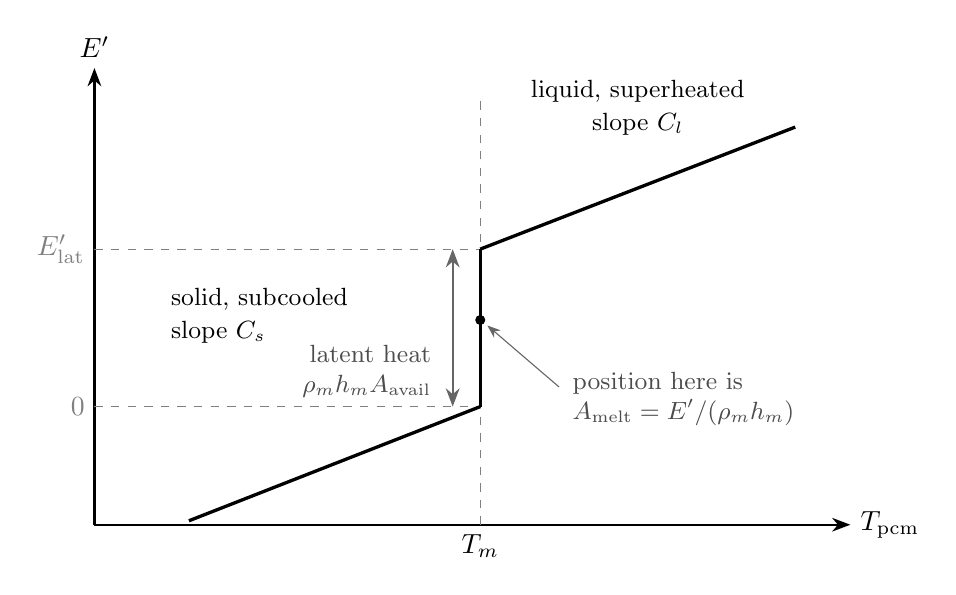
\begin{tikzpicture}[>=Stealth, scale=1.0]
  % axes
  \draw[->,thick] (0,0) -- (9.6,0) node[right] {$T_{\mathrm{pcm}}$};
  \draw[->,thick] (0,0) -- (0,5.8) node[above] {$E'$};
  % melting temperature
  \draw[dashed,gray] (4.9,0) -- (4.9,5.4);
  \node[below] at (4.9,0) {$\Tm$};
  % latent plateau markers
  \draw[dashed,gray] (0,1.5) -- (4.9,1.5) node[pos=0,left] {$0$};
  \draw[dashed,gray] (0,3.5) -- (4.9,3.5) node[pos=0,left] {$E'_{\mathrm{lat}}$};
  % the curve: solid branch, plateau, liquid branch
  \draw[very thick] (1.2,0.05) -- (4.9,1.5);
  \draw[very thick] (4.9,1.5) -- (4.9,3.5);
  \draw[very thick] (4.9,3.5) -- (8.9,5.05);
  % branch labels, all kept clear of the curve and of each other
  \node[align=left,font=\small,anchor=west] at (0.85,2.65)
    {solid, subcooled\\[1pt] slope $C_{s}$};
  \node[align=center,font=\small] at (6.9,5.3)
    {liquid, superheated\\[1pt] slope $C_{l}$};
  % latent plateau annotation, placed to the LEFT of the vertical segment
  \draw[<->,thick,black!60] (4.55,1.5) -- (4.55,3.5);
  \node[font=\small,align=right,anchor=east,black!70] at (4.4,1.95)
    {latent heat\\$\rhom\hm A_{\mathrm{avail}}$};
  % melt-fraction callout, to the RIGHT and well below the liquid branch
  \filldraw (4.9,2.6) circle (1.6pt);
  \draw[->,black!60] (5.9,1.75) -- (4.99,2.53);
  \node[font=\small,align=left,anchor=west,black!70] at (5.95,1.6)
    {position here is\\$\Amelt = E'/(\rhom\hm)$};
\end{tikzpicture}
\caption{The enthalpy curve, Eq.~\eqref{eq:enth-curve}. Reading it as
$E'(T)$ it is multivalued at $\Tm$ --- which is exactly why $T$ cannot be the
state. Reading it as $T(E')$, the direction the code uses, it is single-valued
everywhere. Position on the vertical segment is the melt fraction.}
\label{fig:enthalpy-curve}
\end{figure}

\subsubsection{The state, its capacities, and their sizes}

Let $E'$ be the enthalpy per unit tube length of the PCM belonging to one
segment, measured from a datum of \emph{fully solid at $\Tm$}. The datum is
arbitrary but this choice puts the two branch boundaries at $0$ and
$E'_{\mathrm{lat}}$, which keeps the tests in the code short.

With $A_{\mathrm{avail}}=V_{\mathrm{well}}/(n_{t}L_{\mathrm{tube}})$ the PCM
cross-section a segment actually owns,
\begin{equation}
  E'_{\mathrm{lat}} = \rhom \hm A_{\mathrm{avail}},
  \qquad
  C_{s} = \rhom c_{p,s} A_{\mathrm{avail}},
  \qquad
  C_{l} = \rhom c_{p,l} A_{\mathrm{avail}},
  \label{eq:enth-caps}
\end{equation}
are the latent capacity and the two sensible capacities, all per unit tube
length. Their numerical values at the design point are worth committing to
memory, because they explain the behaviour of the whole formulation:

\begin{center}
\begin{tabular}{@{}l r l@{}}
\toprule
quantity & value & \\
\midrule
$A_{\mathrm{avail}}$      & \num{4.5411e-3} & \si{\meter\squared} \\
$E'_{\mathrm{lat}}$       & \num{2.675}     & \si{\mega\joule\per\meter} \\
$C_{s}$                   & \num{9.010e3}   & \si{\joule\per\meter\per\kelvin} \\
$C_{l}$                   & \num{1.267e4}   & \si{\joule\per\meter\per\kelvin} \\
\midrule
$C_{l}/E'_{\mathrm{lat}}$ & \num{4.74e-3}   & \si{\per\kelvin} \\
\bottomrule
\end{tabular}
\end{center}

\noindent
That last ratio is the Stefan number in disguise. One kelvin of superheat is
worth \SI{0.47}{\percent} of the latent capacity, so the sensible branches are
\emph{energetically} minor --- with the \SI{10}{\kelvin} approach available
here, at most about \SI{4.7}{\percent}. A reader could reasonably conclude that
the whole formulation is a small correction. It is not, and
\S\ref{sec:front:levelling} explains why: the sensible branches matter through
the \emph{driving temperature difference}, not through the energy they store.

The enthalpy curve and the melted area follow directly:
\begin{equation}
  T_{\mathrm{pcm}} =
  \begin{dcases}
    \Tm + E'/C_{s}, & E' < 0 \quad\text{(solid, subcooled)},\\[2pt]
    \Tm, & 0 \le E' \le E'_{\mathrm{lat}} \quad\text{(two-phase)},\\[2pt]
    \Tm + \bigl(E'-E'_{\mathrm{lat}}\bigr)/C_{l},
      & E' > E'_{\mathrm{lat}} \quad\text{(liquid, superheated)},
  \end{dcases}
  \qquad
  \Amelt = \frac{\min\!\left(\max(E',0),\,E'_{\mathrm{lat}}\right)}{\rhom \hm}.
  \label{eq:enth-curve}
\end{equation}

The clipping in $\Amelt$ is not a guard bolted on to prevent bad behaviour ---
it is the definition. Melted area saturates because a segment cannot melt PCM it
does not own, and superheat is where the extra energy goes. This is the sense in
which $\varepsilon_{\mathrm{local}}\in[0,1]$ is \emph{structural} in
Formulation~C: there is no code path that can violate it, so no test is needed.

\subsubsection{The segment equation, derived}
\label{sec:front:segeq}

Equation~\eqref{eq:enth-ode} below is the heart of the march, and it is short
enough to look like a definition. It is not: it is the result of writing an
energy balance on two different control volumes and then eliminating the
quantity they share. This subsection does that in full, because the conductance
$K$ that comes out is \emph{not} the $\Ui P_{i}$ a reader would write down
unaided, and the difference reaches \SI{33}{\percent} at this design point.

\paragraph{The two control volumes.}
Fix a segment $j$, spanning $z\in[z_{j},z_{j+1}]$ with $\Delta z =
z_{j+1}-z_{j}$. Two control volumes share the tube wall over that interval:

\begin{description}[leftmargin=1.9em,itemsep=2pt]
\item[CV\,1 --- the PCM] belonging to segment $j$: cross-section
  $A_{\mathrm{avail}}$, length $\Delta z$, stationary, closed.
\item[CV\,2 --- the fluid] inside the tube over the same interval:
  cross-section $A_{\mathrm{flow}}=\pi r_{i}^{2}$, open, with mass flow $\md$
  entering at $T_{j}$ and leaving at $T_{j+1}$.
\end{description}

\noindent
Write $q'_{j}$ for the heat per unit tube length crossing from CV\,2 into
CV\,1. It appears in both balances with opposite sign, and eliminating it is
the whole exercise.

\medskip
\noindent\textbf{Step 1 --- the PCM balance.}
CV\,1 is closed and stationary, so the first law reduces to a statement about
its enthalpy alone. With $E'$ the enthalpy per unit tube length
(\S\ref{sec:front:enthalpy}), the enthalpy of the control volume is
$E'\Delta z$ and
\begin{equation}
  \frac{\mathrm{d}}{\mathrm{d}t}\bigl(E'_{j}\,\Delta z\bigr)
  \;=\;
  \underbrace{q'_{j}\,\Delta z}_{\text{through the tube wall}}
  \;\underbrace{-\;\bigl[\dot Q_{\mathrm{ax}}\bigr]_{z_{j}}^{z_{j+1}}}
              _{\text{axial conduction, H2}}
  \;+\;\underbrace{\dot Q_{\mathrm{form}}}_{\text{formation, H6}}
  \;+\;\underbrace{\dot Q_{\mathrm{azi}}}_{\text{neighbours, H9}} ,
\end{equation}
and the last three terms are dropped by hypothesis. Two of those deletions are
worth a number rather than a citation:

\begin{itemize}[leftmargin=1.5em,itemsep=2pt]
\item \textbf{Axial conduction (H2)} is negligible by an enormous margin. The
  axial diffusion time over one segment is $\Delta z^{2}/\alpha_{l} =
  \SI{5.4e9}{\second}$ against a \SI{3.6e4}{\second} charging window --- a ratio
  of $1.5\times10^{5}$. With $\Delta z = \SI{30.5}{\meter}$ this is not a close
  call, and it would remain safe at a hundred times the segment count.
\item \textbf{Azimuthal conduction (H9)} is \emph{not} negligible and is
  assumed away pending the calculation described in \S\ref{sec:defects:h9}. At
  the wellhead the neighbouring cell is \SI{48.9}{\kelvin} away and a slab
  estimate gives $\sim\SI{22}{\watt\per\meter}$ against a useful duty of
  $\sim\SI{83}{\watt\per\meter}$. This is the least defensible term in the
  model.
\end{itemize}

\noindent
Dividing by $\Delta z$ leaves the PCM balance in the form used by the code:
\begin{equation}
  \boxed{\;\frac{\mathrm{d}E'_{j}}{\mathrm{d}t} \;=\; q'_{j}\;}
  \label{eq:pcm-balance}
\end{equation}

\medskip
\noindent\textbf{Step 2 --- the fluid balance.}
CV\,2 is open. For incompressible single-phase flow (H7) with no viscous
dissipation, the energy equation per unit tube length is
\begin{equation}
  \underbrace{\rho A_{\mathrm{flow}} c_{p}\,\frac{\partial T}{\partial t}}
             _{\text{fluid thermal inertia}}
  \;+\;
  \md\,c_{p}\,\frac{\partial T}{\partial z}
  \;=\;
  -\,q'(z) .
  \label{eq:fluid-pde}
\end{equation}

The model drops the first term, and this deserves justification rather than
assertion. Two comparisons, pointing the same way:

\begin{center}
\begin{tabular}{@{}l r l@{}}
\toprule
fluid transit time over $L_{\mathrm{tube}}$ & \SI{2264}{\second} & ($u=\SI{1.35}{\meter\per\second}$) \\
charging window $t_{\mathrm{ch}}$           & \SI{36000}{\second} & \\
\midrule
ratio                                        & \num{0.063} & \\
$\rho A_{\mathrm{flow}}c_{p} \,/\, C_{l}$    & \num{0.257} & fluid vs.\ PCM sensible capacity \\
$\rho A_{\mathrm{flow}}c_{p}\Delta T \,/\, E'_{\mathrm{lat}}$
   & \num{0.0122} & fluid swing vs.\ PCM latent, $\Delta T=\SI{10}{\kelvin}$ \\
\bottomrule
\end{tabular}
\end{center}

\noindent
The fluid re-establishes its profile in one transit, $\SI{2264}{\second}$,
while the PCM state evolves over \SI{10}{\hour}: a $16\times$ separation, so
quasi-steady is reasonable but \emph{not} asymptotic. The honest reading is
that the first \SI{38}{\minute} of each half-cycle is a startup transient the
model does not resolve, worth about \SI{6}{\percent} of the window. What makes
this tolerable is the third row: the energy parked in the fluid is only
\SI{1.2}{\percent} of the latent inventory it is charging, so the transient
misplaces very little energy even though it lasts a noticeable fraction of the
run.

Setting $\partial T/\partial t = 0$ and using the fact that CV\,1 presents a
\emph{single} temperature $T_{\mathrm{pcm}}$ to the whole segment
(H5, the lumped state of \S\ref{sec:front:enthalpy}), the driving difference is
$T(z)-T_{\mathrm{pcm}}$ and the local flux closes on the network of
\S\ref{sec:network}:
\begin{equation}
  q'(z) \;=\; \Ui\,\bigl(2\pi r_{i}\bigr)\,\bigl[T(z)-T_{\mathrm{pcm}}\bigr].
  \label{eq:local-flux}
\end{equation}
Note that $2\pi r_{i}$ appears, not $P_{T}$: $\Ui$ was referred to the
\emph{inner} area in Eq.~\eqref{eq:Ui}, and the finned perimeter is already
inside it through $R'_{\mathrm{outer}}$. Using $P_{T}$ here would count the fins
twice --- which is a compact statement of the v0.1 defect.

\medskip
\noindent\textbf{Step 3 --- integrate across the segment.}
Substituting Eq.~\eqref{eq:local-flux} into the steady form of
Eq.~\eqref{eq:fluid-pde} gives a linear ODE in $z$ with $T_{\mathrm{pcm}}$ and
$\Ui$ held constant over the segment:
\begin{equation}
  \md c_{p}\frac{\mathrm{d}T}{\mathrm{d}z}
  = -2\pi r_{i}\Ui\bigl(T-T_{\mathrm{pcm}}\bigr)
  \quad\Longrightarrow\quad
  \frac{\mathrm{d}\bigl(T-T_{\mathrm{pcm}}\bigr)}{T-T_{\mathrm{pcm}}}
  = -\frac{2\pi r_{i}\Ui}{\md c_{p}}\,\mathrm{d}z .
\end{equation}
Integrating from $z_{j}$ to $z_{j+1}$,
\begin{equation}
  T_{j+1} \;=\; T_{\mathrm{pcm}}
    + \bigl(T_{j}-T_{\mathrm{pcm}}\bigr)e^{-\mathrm{NTU}_{j}},
  \qquad
  \mathrm{NTU}_{j} \;=\; \frac{2\pi r_{i}\,\Ui\,\Delta z}{\md\,c_{p}},
  \label{eq:ntu-derived}
\end{equation}
which is Eq.~\eqref{eq:ntu}. It is the single-stream heat-exchanger result: one
stream with finite capacity rate $\md c_{p}$, the other an isothermal reservoir
of infinite capacity rate, effectiveness $\varepsilon = 1-e^{-\mathrm{NTU}}$.
The reservoir idealisation is exactly what the lumped PCM state licenses.

\medskip
\noindent\textbf{Step 4 --- the closure.}
The heat the fluid actually gives up over the segment is the enthalpy it loses,
\begin{equation}
  q'_{j}\,\Delta z \;=\; \md c_{p}\bigl(T_{j}-T_{j+1}\bigr)
  \;\overset{\eqref{eq:ntu-derived}}{=}\;
  \md c_{p}\bigl(T_{j}-T_{\mathrm{pcm}}\bigr)\bigl(1-e^{-\mathrm{NTU}_{j}}\bigr),
\end{equation}
and dividing by $\Delta z$ gives the conductance that closes
Eq.~\eqref{eq:pcm-balance}:
\begin{equation}
  \boxed{\;
  q'_{j} = K_{j}\bigl(T_{j}-T_{\mathrm{pcm}}\bigr),
  \qquad
  K_{j} = \frac{\md\,c_{p}\bigl(1-e^{-\mathrm{NTU}_{j}}\bigr)}{\Delta z} .
  \;}
  \label{eq:K-derived}
\end{equation}

Combining Eqs.~\eqref{eq:pcm-balance} and \eqref{eq:K-derived} with the
enthalpy curve $T_{\mathrm{pcm}}(E')$ of Eq.~\eqref{eq:enth-curve} closes the
system. This is the segment equation:
\begin{equation}
  \boxed{\;
  \frac{\mathrm{d}E'}{\mathrm{d}t}
  \;=\; K\left(T_{j} - T_{\mathrm{pcm}}(E')\right),
  \qquad
  K = \frac{\md\,c_{p}\left(1-e^{-\mathrm{NTU}}\right)}{\Delta z}.
  \;}
  \label{eq:enth-ode}
\end{equation}

One unknown per segment, $E'$; everything else is either geometry, a property,
or the upstream fluid temperature $T_{j}$ handed down by the segment before it.

\paragraph{Why $K$ is not $\Ui P_{i}$.}
This is the step most easily got wrong, so it is worth isolating. The naive
closure takes Eq.~\eqref{eq:local-flux} with $T(z)\approx T_{j}$, giving
$q'_{j}\approx 2\pi r_{i}\Ui (T_{j}-T_{\mathrm{pcm}})$. Comparing:
\begin{equation}
  \frac{K_{j}}{2\pi r_{i}\Ui}
  \;=\;
  \frac{1-e^{-\mathrm{NTU}_{j}}}{\mathrm{NTU}_{j}}
  \;\le\; 1 .
  \label{eq:K-ratio}
\end{equation}
The two limits say what the difference means:

\begin{description}[leftmargin=1.9em,itemsep=3pt]
\item[$\mathrm{NTU}\to0$:] the ratio $\to1$. The fluid barely cools across the
  segment, $T(z)\approx T_{j}$ throughout, and the naive closure is right.
\item[$\mathrm{NTU}\to\infty$:] $K\to \md c_{p}/\Delta z$, a finite limit set
  by the \emph{fluid}, not the wall. No matter how good the borehole is, a
  segment cannot absorb more than the stream can carry to it. The naive closure
  has no such limit and would let $T_{j+1}$ fall below $T_{\mathrm{pcm}}$ ---
  heat flowing from cold to hot, at a rate that grows without bound as $\Ui$
  improves.
\end{description}

\noindent
At this design point $\mathrm{NTU}$ runs from \num{0.083} to \num{0.602} over
the charge, so Eq.~\eqref{eq:K-ratio} lies between \num{0.96} and \num{0.75}:
\textbf{using $\Ui P_{i}$ would overstate the conductance by \SI{4}{\percent}
to \SI{33}{\percent}}, worst where the melt layer is thinnest and the borehole
best. The error is largest exactly where the model is most active, which is why
it cannot be waved away as second order.

\paragraph{Two properties inherited from this derivation.}

\begin{description}[leftmargin=1.9em,itemsep=3pt]
\item[Closure is structural.] The code does not evaluate
  Eq.~\eqref{eq:K-derived} and Eq.~\eqref{eq:pcm-balance} independently. It
  integrates Eq.~\eqref{eq:pcm-balance} over the step and \emph{reports}
  $q'_{j}=(E'^{\,n+1}-E'^{\,n})/\Delta t$, then drops the fluid temperature by
  exactly that amount, $T_{j+1}=T_{j}-q'_{j}\Delta z/(\md c_{p})$. Whatever the
  PCM gained, the fluid lost, to machine precision, with no possibility of
  drift.
\item[$K$ is frozen over a time step, $T_{\mathrm{pcm}}$ is not.] $K_{j}$ is
  evaluated once per step from the melt thickness at the start of it, whereas
  $T_{\mathrm{pcm}}$ is advanced exactly inside the step by
  Eq.~\eqref{eq:enth-exact}. The consequence is that $T_{j+1}$ equals the
  $\varepsilon$--NTU result of Eq.~\eqref{eq:ntu-derived} only while the segment
  is on the latent plateau, where $T_{\mathrm{pcm}}=\Tm$ is genuinely constant.
  In the sensible branches the two differ at second order in $\Delta t$. This
  is a deliberate choice: it keeps closure exact, which matters more than
  matching an $\varepsilon$--NTU relation that is itself only quasi-steady.
\end{description}

Two properties of Eq.~\eqref{eq:enth-ode} drive everything that follows:

\begin{itemize}[leftmargin=1.5em,itemsep=2pt]
\item It is \textbf{nonlinear}, because $T_{\mathrm{pcm}}(E')$ is piecewise.
\item It is \textbf{linear inside each branch}, because each piece of
  Eq.~\eqref{eq:enth-curve} is affine in $E'$.
\end{itemize}

\noindent
The second property is what makes an exact integration possible, and
\S\ref{sec:front:integration} takes it up. But first, why an exact integration
is not optional.

\subsubsection{Why explicit stepping fails --- and why nobody noticed until v0.4}
\label{sec:front:integration}

Look again at the three branches. On the plateau, $T_{\mathrm{pcm}}=\Tm$ is
\emph{constant}: it does not respond to $E'$ at all. The segment therefore
behaves as though it had infinite heat capacity, Eq.~\eqref{eq:enth-ode} reduces
to $\mathrm{d}E'/\mathrm{d}t = \text{constant}$, and an explicit Euler step is
not merely stable but \emph{exact}.

This is precisely the regime Formulations A and B live in permanently. Explicit
stepping was safe in v0.1 and v0.2 for a structural reason, not a lucky one ---
and that is why the time grid was never examined.

Add the sensible branches and the capacity becomes finite. Equation
\eqref{eq:enth-ode} is now a relaxation equation with time constant $C/K$, and
explicit Euler requires $\Delta t < C/K$. At the design point:

\begin{center}
\begin{tabular}{@{}l r r@{}}
\toprule
 & early ($t=\SI{1}{\second}$) & late ($t\to t_{ch}$) \\
\midrule
$\mathrm{NTU}$, segment 1        & \num{0.592}  & \num{0.083} \\
$K$ \si{[\watt\per\meter\per\kelvin]} & \num{64.3} & \num{11.5} \\
$C_{l}/K$ \si{[\second]}         & \num{197}    & \num{1106}  \\
time-grid step $\Delta t$ \si{[\second]} & \num{0.31} & \num{8491} \\
\midrule
$\Delta t\,K/C_{l}$              & \num{0.002}  & \textbf{\num{7.7}} \\
\bottomrule
\end{tabular}
\end{center}

\noindent
The grid is logarithmic, so it is fine at the start and violates the limit by
almost an order of magnitude at the end. The first implementation duly
diverged: the oscillation fed back through the fluid temperature and drove the
secondary fluid to \SI{261}{\kelvin}, some \SI{170}{\kelvin} below anything
physical.

This is a good failure to have seen once. It was loud, it was immediate, and it
was diagnosable. The dangerous version of the same error is a step ratio of
$1.5$ rather than $7.7$: still unstable in principle, but slowly enough to look
like a plausible answer.

\subsubsection{Branchwise-exact integration}

Rather than shrink $\Delta t$ --- which would multiply the cost of every run by
$\sim\!10^{3}$ --- exploit the linearity within each branch and integrate in
closed form. Holding the fluid temperature $T_{j}$ fixed across the step:

\begin{equation}
  \underbrace{E'(t+\Delta t) = E' + K\left(T_{j}-\Tm\right)\Delta t}
             _{\text{plateau: linear}},
  \qquad
  \underbrace{E'(t+\Delta t) = E'_{\mathrm{eq}}
    + \bigl(E'-E'_{\mathrm{eq}}\bigr)e^{-K\Delta t/C}}
             _{\text{sensible: exponential relaxation}},
  \label{eq:enth-exact}
\end{equation}

\noindent
with the equilibrium enthalpy and the relevant capacity
\begin{equation}
  \left(C,\;E'_{\mathrm{eq}}\right) =
  \begin{cases}
    \left(C_{s},\; C_{s}\left(T_{j}-\Tm\right)\right), & E' < 0,\\[3pt]
    \left(C_{l},\; E'_{\mathrm{lat}} + C_{l}\left(T_{j}-\Tm\right)\right),
      & E' > E'_{\mathrm{lat}}.
  \end{cases}
\end{equation}

$E'_{\mathrm{eq}}$ is the enthalpy at which the PCM would sit in equilibrium
with the fluid --- the state the segment relaxes toward and never quite reaches.
The exponential is unconditionally stable and monotone: no step size, however
large, can overshoot it. That is the property explicit Euler lacks.

\paragraph{Crossing a branch boundary.}
A step may start in one branch and end in another. The step is then split at the
crossing. Let $E'_{b}$ be the boundary being approached ($0$ or
$E'_{\mathrm{lat}}$). The crossing time is
\begin{equation}
  t^{*} =
  \begin{dcases}
    \frac{E'_{b}-E'}{K\left(T_{j}-\Tm\right)}, & \text{from the plateau},\\[8pt]
    \frac{C}{K}\,
      \ln\!\left(\frac{E'-E'_{\mathrm{eq}}}{E'_{b}-E'_{\mathrm{eq}}}\right),
      & \text{from a sensible branch},
  \end{dcases}
  \label{eq:crossing}
\end{equation}
and if $t^{*} < \Delta t$ the state is advanced to $E'_{b}$, the remaining
$\Delta t - t^{*}$ is integrated in the adjacent branch, and the test is
repeated. At most a handful of crossings can occur in one step, so the loop is
bounded.

The heat reported to the fluid is then
\begin{equation}
  q'_{j} = \frac{E'^{\,n+1}-E'^{\,n}}{\Delta t},
  \label{eq:qfromE}
\end{equation}
\emph{by definition}, not by a separate flux evaluation. Whatever the segment
gained, the fluid lost. Closure is exact to machine precision and cannot drift.

\begin{worked}[A bug worth studying: the sticky boundary]
The branch test in the code is written with closed intervals,
$0 \le E' \le E'_{\mathrm{lat}}$, so a state landing \emph{exactly} on
$E'_{\mathrm{lat}}$ is still classified as two-phase. Follow the logic: the
plateau branch computes $t^{*} = (E'_{\mathrm{lat}} - E')/\text{rate} = 0$,
finds $t^{*} < \Delta t$, advances the state to $E'_{\mathrm{lat}}$ ---
where it already is --- and subtracts zero from the remaining time. The next
iteration does the same. The segment is pinned at the boundary for ever and
never enters the liquid branch.

The symptom was not a crash. It was every segment reporting a melt fraction of
exactly $1.000$ and a superheat of exactly zero --- results that look
\emph{excellent}. The tell was a single diagnostic line printing ``sensible
energy stored: \num{0.000}'', a quantity that had no business being identically
zero.

The fix is to step just past the boundary rather than onto it,
\[
  E' \leftarrow E'_{\mathrm{lat}} + \epsilon,
  \qquad \epsilon = 10^{-9}\max\!\left(E'_{\mathrm{lat}},1\right),
\]
so the next iteration selects the liquid branch. The general lesson: when a
solver switches on the sign of a quantity, decide deliberately which side of the
boundary the equality belongs to, and make sure the state cannot come to rest
on it.
\end{worked}

\paragraph{Verification.}
The scheme was checked against a brute-force explicit integration of
Eq.~\eqref{eq:enth-ode} using \num{200000} substeps, over a charge and a
discharge, including steps that cross branch boundaries. Agreement is
$3\times10^{-13}$ relative --- machine precision. This is a genuine
verification: the two calculations share no code path beyond
Eq.~\eqref{eq:enth-curve}.

\subsubsection{Recovering the melt-layer thickness}

The resistance network needs $\delta$, not $\Amelt$. Inverting
Eq.~\eqref{eq:area-fins} --- which excludes the fin metal from the melted PCM
--- gives $\delta$ as described in \S\ref{sec:front:finmetal}, and the network
of \S\ref{sec:network} is otherwise unchanged in form.

One thing \emph{is} changed: the driving temperature. In Formulations~A and~B
the outer boundary of the resistance chain sits at $\Tm$. In Formulation~C it
sits at $T_{\mathrm{pcm}}$, which equals $\Tm$ only while some solid remains.
This single substitution is the mechanism of the next subsection.

\subsubsection{Sensible heat is self-levelling}
\label{sec:front:levelling}

Here is why a \SI{4.7}{\percent} energy term produces a first-order change in
the answer.

Consider again the well-head segment that melts first. Under Formulation~B it
finished melting and then continued to absorb heat at the full driving
difference $T_{j}-\Tm$, because its boundary temperature was pinned at $\Tm$
regardless of state. It monopolised the fluid's heat. The segments downstream,
which had not finished, received whatever was left.

Under Formulation~C the same segment starts to superheat the instant its solid
is gone. $T_{\mathrm{pcm}}$ rises, $T_{j}-T_{\mathrm{pcm}}$ collapses, its
demand falls away, and the heat continues down the well to segments that still
have solid to melt. The mechanism is a negative feedback, and it is automatic:
nothing in the code distributes the heat, and no parameter was tuned.

The effect on the distribution of melt is large:

\begin{center}
\begin{tabular}{@{}l l r@{}}
\toprule
formulation & $\varepsilon_{\mathrm{local}}$ at ten stations & spread \\
\midrule
B (latent only) & 1.78\; 0.73\; 0.69\; 0.71\; 0.77\; 0.85\; 0.94\; 1.03\; 1.12\; 1.23 & 1.321 \\
C (enthalpy)    & 1.00\; 1.00\; 1.00\; 1.00\; 1.00\; 1.00\; 1.00\; 1.00\; 1.00\; 1.00 & \textbf{0.078} \\
\bottomrule
\end{tabular}
\end{center}

\noindent
where the spread is
$\max_{j}\varepsilon_{\mathrm{local}}-\min_{j}\varepsilon_{\mathrm{local}}$ over
the \num{100} segments at end of charge. Two separate things improved. The
values above $1$ are gone, because Eq.~\eqref{eq:enth-curve} makes them
impossible. The values well below $1$ are gone too, and that is the physical
result: PCM that never melts is \emph{dead volume} --- it occupies borehole,
costs money, and carries no energy through the round trip. Formulation~C says
there is far less of it than Formulation~B implied.

\subsubsection{What Formulation C still does not do}

Three limitations, stated plainly because they bound how far the result can be
pushed.

\begin{description}[leftmargin=1.7em,itemsep=3pt]
\item[One temperature per segment.] $E'$ is a lumped quantity: all the PCM in a
  segment is at a single $T_{\mathrm{pcm}}$. There is no radial resolution
  \emph{within} a phase, so superheat appears instantaneously and uniformly
  across the whole liquid annulus rather than diffusing outward from the tube.
  The model therefore reaches its superheated state sooner than the real
  material would, and the self-levelling above is an upper bound on the effect.
\item[H1 is inherited, not repaired.] The quasi-steady melt layer of
  \S\ref{sec:front:legacy} is still assumed: the conduction profile through the
  liquid is taken as instantaneously steady. This is justified by
  $\mathrm{Ste}=\num{0.047}$ and is a good approximation here, but it is an
  approximation, and it is the same one in all three formulations.
\item[H3 is now \emph{saturated}.] Because $\varepsilon_{\mathrm{local}}\to1$
  over essentially the whole well, $\delta \to \delta_{\mathrm{merge}}$
  everywhere --- the melt fronts of neighbouring legs are touching. The annular
  conduction resistance is being evaluated at the exact limit of its validity.
  \S\ref{sec:defects:h3} takes this up, because it now carries a design
  decision.
\end{description}

Formulation~C is nonetheless the first of the three that is \emph{closed}: every
joule the resistance network delivers has a place to go, and the melt fraction
cannot leave $[0,1]$. Whatever is wrong with the answer is now wrong in the heat
transfer, not in the bookkeeping.

\emph{Source:} \code{pcm\_capacities}, \code{pcm\_state},
\code{advance\_segment}, \code{march\_h}.

%---------------------------------------------------------------------
\subsection{Latent inventory and the melted fraction}
\label{sec:front:inventory}

The melted volume per tube and the melted fraction of the borehole inventory are
\begin{equation}
  \Vmelt \;=\; \sum_{j=1}^{n_{s}} \Amelt^{(j)}\,\Delta z,
  \qquad
  \varepsilon_{\mathrm{PCM}}
  \;=\;
  \frac{\Vmelt\, n_{t}}{V_{\mathrm{well}}},
  \label{eq:eps}
\end{equation}
with $V_{\mathrm{well}}$ from Eq.~\eqref{eq:Vwell} and the multiplier $n_{t}$,
not $2n_{t}$, for the reason given after Eq.~\eqref{eq:Ltube}.

The density $\rhom$ in Eqs.~\eqref{eq:marched}--\eqref{eq:qeff} is the
\emph{same in both directions}, and is taken as the solid density $\rho_{s}$.
The thermal conductivity $\km$ by contrast \emph{is} directional, $k_{l}$ while
melting and $k_{s}$ while freezing, because the layer adjacent to the tube is
liquid in the first case and solid in the second.

The asymmetry is deliberate. Making the latent inventory directional as well
would bank energy at $\rho_{l}$ and return it at $\rho_{s}$, yielding
$\rho_{s}/\rho_{l}=1.069$ times more energy out than in --- a \SI{6.9}{\percent}
round-trip gain from bookkeeping alone. Carrying the front as a
\emph{solid-equivalent} area instead makes $\varepsilon_{\mathrm{PCM}}$ a true
melted \emph{mass} fraction and makes stored energy equal to available energy.
The price is that the \SI{6.9}{\percent} volume change on melting is not
represented: the liquid layer is about \SI{2.3}{\percent} thicker in radius than
Eq.~\eqref{eq:area-fins} reports, so Eq.~\eqref{eq:he} mildly under-predicts the
melt-layer resistance.

\emph{Source:} \code{thums\_core/stefan.py}; \code{config.PCM.rho\_latent}.

%=====================================================================
\section{Hydraulics, well-field sizing and performance indices}
\label{sec:hydraulics}

%---------------------------------------------------------------------
\subsection{Pressure drop and pumping power}
\label{sec:hydraulics:dp}

Properties are evaluated at the mean of the inlet and outlet temperatures. With
the flow area $A_{\mathrm{flow}}=\pi r_{i}^{2}$,
\begin{equation}
  u \;=\; \frac{\md}{\rho A_{\mathrm{flow}}},
  \qquad
  \mathrm{Re} \;=\; \frac{\rho\,u\,D_{i}}{\mu},
\end{equation}
and the Darcy friction factor is taken as laminar or Blasius,
\begin{equation}
  f =
  \begin{dcases}
    \dfrac{64}{\mathrm{Re}}, & \mathrm{Re} < 2000, \\[6pt]
    \dfrac{0.3164}{\mathrm{Re}^{1/4}}, & \mathrm{Re} \leq 10^{5},
  \end{dcases}
  \label{eq:friction}
\end{equation}
giving the Darcy--Weisbach frictional drop
\begin{equation}
  \Delta p_{\mathrm{fric}}
  \;=\; f\,\frac{L_{\mathrm{tube}}}{D_{i}}\,\frac{\rho u^{2}}{2} .
  \label{eq:dp-fric}
\end{equation}

Minor losses are added with a lumped coefficient for one hairpin --- a
sharp-edged entrance, two $180^{\circ}$ return bends and an exit:
\begin{equation}
  K_{\mathrm{tot}}
  \;=\; K_{\mathrm{ent}} + 2K_{\mathrm{bend}} + K_{\mathrm{exit}}
  \;=\; 0.5 + 2(2.2) + 1.0 \;=\; 5.9,
  \qquad
  \Delta p_{\mathrm{min}} \;=\; K_{\mathrm{tot}}\,\frac{\rho u^{2}}{2} .
  \label{eq:dp-minor}
\end{equation}
The total drop and the hydraulic power for one tube are then
\begin{equation}
  \Delta p \;=\; \Delta p_{\mathrm{fric}} + \Delta p_{\mathrm{min}},
  \qquad
  \dot W_{\mathrm{pump,tube}} \;=\; \frac{\md\,\Delta p}{\rho} .
  \label{eq:dp}
\end{equation}

The three coefficients in Eq.~\eqref{eq:dp-minor} are hard-coded literals rather
than configuration parameters, and the source describes them as example values.
They are not derived from the completion geometry and cannot be varied from
\code{Case}. At the design point $\Delta p_{\mathrm{min}}$ is small beside
$\Delta p_{\mathrm{fric}}$ because $L_{\mathrm{tube}}/D_{i}\approx 10^{5}$, but
the asymmetry is worth knowing: any sensitivity study on pumping power is
varying only the friction term.
The field total scales by the tube and well counts,
\begin{equation}
  \dot W_{\mathrm{pump}}
  \;=\;
  \dot W_{\mathrm{pump,tube}}\; n_{t}\,\Nwells .
\end{equation}

Two properties of Eq.~\eqref{eq:friction} deserve note. The smooth-tube
assumption sets the roughness to zero, which is optimistic for a well
completion. And no correlation is supplied above $\mathrm{Re}=10^{5}$; the
Blasius branch is simply extrapolated, which is where discharge cases with
elevated flow will land.

\emph{Source:} \code{\_legacy\_physics.calculate\_pressure\_drop}.

%---------------------------------------------------------------------
\subsection{Well-field sizing}
\label{sec:hydraulics:sizing}

\subsubsection*{The v0.1 criterion}

v0.1 sized the field on a single requirement: that the wells absorb the charging
energy within the charging window. Writing $\Delta E_{\mathrm{del}}(\Nwells)$ for
the energy the field takes up over $t_{\mathrm{ch}}$,
\begin{equation}
  \Phi_{\mathrm{heat}}(\Nwells)
  \;\equiv\;
  \frac{\Delta E_{\mathrm{out,HP}}}{\Delta E_{\mathrm{del}}(\Nwells)} - 1
  \;=\; 0 .
  \label{eq:N-heat}
\end{equation}
This is a rate question. Nothing in v0.1 required the wells to \emph{contain}
enough PCM to hold that energy.

\subsubsection*{The capacity criterion}
\label{sec:hydraulics:capacity}

The missing requirement is that the field be able to \emph{contain} the energy
at all, not merely absorb it fast enough:
\begin{equation}
  \boxed{\;
  \Nwells \;=\; \max\bigl(N_{\mathrm{charge\ rate}},\; N_{\mathrm{capacity}}\bigr),
  \qquad
  N_{\mathrm{capacity}}
  = \frac{\Delta E_{\mathrm{out,HP}}}{E_{\mathrm{well}}},
  \;}
  \label{eq:sizing}
\end{equation}
with the capacity of one well written, as in the v0.1 notebook, from latent
\emph{and} sensible heat:
\begin{equation}
  E_{\mathrm{well}}
  = \rhom V_{\mathrm{well}}
    \left[\hm + c_{p,l}\left(T_{3c}-\Tm\right)\right].
  \label{eq:E-well}
\end{equation}
The sensible term is the zero-resistance limit: with no thermal resistance the
liquid would reach the charging inlet temperature. Equation~\eqref{eq:E-well} is
closed form, so unlike the constraint it replaces it costs nothing to evaluate.

This is the quantity the v0.1 notebook computed as \code{N\_wells\_ideal} and
then spent only on costing. In v0.3 its place was taken by a melted-volume
condition, $\varepsilon_{\mathrm{PCM}}(N)=1$, which on inspection was not a
capacity statement at all but ``the well count at which an unthrottled
\SI{10}{\hour} charge exactly saturates the store'' --- a strange thing to size
on, and one that allowed the field to over-charge by \SI{7}{\percent} relative
to the requirement.

Which criterion binds depends on the wall conductivity. With the legacy value
the rate criterion dominates, which is why the omission stayed invisible for so
long. With the correct steel conductivity the rate requirement collapses and
capacity takes over.

\subsubsection*{A reporting rule: $N_{\mathrm{capacity}}$ is a bound, not a result}

Equation~\eqref{eq:sizing} is a maximum, and that has a consequence for how its
parts may be read. $N_{\mathrm{capacity}}$ is the seductive one --- it is closed
form, it is smooth, it responds to every geometric parameter, and \emph{it is
wrong to read on its own}. Whenever the rate criterion binds,
$N_{\mathrm{capacity}}$ moves while the answer does not, and it can move the
opposite way.

The failure is not hypothetical; \S\ref{sec:defects:h3} records a fin sweep in
which $N_{\mathrm{capacity}}$ falls monotonically while $\Nwells$ rises by
\SI{42}{\percent}. Two properties of Eq.~\eqref{eq:E-well} explain it:
$E_{\mathrm{well}} \propto V_{\mathrm{well}}$, and $V_{\mathrm{well}}$ counts
whatever the metal does not occupy --- so $N_{\mathrm{capacity}}\cdot
V_{\mathrm{well}}$ is invariant under any change to the fins, and the column is
pure volume bookkeeping.

The model therefore reports through \code{sizing\_report}, which leads with
$\Nwells$, names the criterion that set it, gives the margin by which the other
is slack, and labels $N_{\mathrm{capacity}}$ as a lower bound. At the design
point the margin is \SI{2.6}{\percent}: the design sits \emph{on} the crossover,
so any parameter sweep switches criterion partway through, and the report warns
when this is so.

\subsubsection*{Why the field is not sized on the discharge}

It is natural to ask whether $\Nwells$ should instead be converged on the
discharge --- the duty that must actually be met --- with the flow converged on
the charge. It cannot, and the reason is structural: \emph{sizing must act on
whichever variable is free.}

During charging the flow is pinned by the specified glide,
$\mdw^{\mathrm{ch}} = \dot Q_{\mathrm{out,HP}}/(c_{p,w}\Delta T_{3C,2C})$, so
$\Nwells$ is the only freedom and the charge can size it. During discharging
$\Nwells$ is already fixed, so the flow is the freedom and the discharge sizes
that instead.

Pinning the discharge flow to its own glide as well --- $\Delta T_{2D,3D}$ is
tied to $\Delta T_{3C,2C}$ by Eq.~\eqref{eq:glide-tied} --- over-determines the
problem, and measurably so:

\begin{center}
\begin{tabular}{@{}r r r@{}}
\toprule
$\Nwells$ & $\varepsilon_{\mathrm{PCM}}$ & $\Delta E_{\mathrm{dc}}/\Delta E_{\mathrm{in,ORC}}$ \\
\midrule
 8    & 1.505 & 0.9285 \\
12.74 & 0.999 & 0.9776 \\
18    & 0.719 & 0.9925 \\
24    & 0.541 & 0.9960 \\
40    & 0.325 & 0.9962 \\
\bottomrule
\end{tabular}
\end{center}

\noindent The delivered energy saturates at $0.996$ and never reaches unity for
\emph{any} well count, because the fluid leaves slightly short of the nominal
outlet temperature and so carries about \SI{0.4}{\percent} less energy per unit
mass than $c_{p}\Delta T$ presumes. There is no root. Letting the discharge flow
float by the required \SI{1.3}{\percent} is precisely what the flow loop exists
to do, and the v0.1 arrangement is therefore correct and is retained.

\subsubsection*{Comparison with the v0.1 ideal well count}
\label{sec:hydraulics:ideal}

The v0.1 notebook printed \code{Ideal number of wells: 12.215} from
\begin{equation}
  m_{\mathrm{ideal}}
  = \frac{\Delta E_{\mathrm{out,HP}}}{\hm + c_{p,l}\left(T_{3c}-\Tm\right)},
  \qquad
  m_{\mathrm{well}} = V_{\mathrm{well}}\,\rho_{l},
  \label{eq:N-ideal-v01}
\end{equation}
which is Eq.~\eqref{eq:E-well} with $\rho_{l}$ in place of $\rhom$. It carries
no thermal resistance and no losses, so it is a genuine \textbf{lower bound}:
the best any design could achieve. Designs with high
$\varepsilon_{\mathrm{PCM}}$ are desirable precisely because they approach it
--- the PCM in the ground is being used rather than merely occupying the
borehole.

\medskip
\noindent\textbf{Correction to version 0.3 of this document.} v0.3 stated that
$N_{\mathrm{inventory}}/N_{\mathrm{ideal}} = 1.0428$ agreed with
$1+\mathrm{Ste} = 1.0474$, and attributed the gap to the sensible heat the model
then omitted. That comparison was made on \emph{inconsistent bases} and the
agreement was a coincidence. Equation~\eqref{eq:N-ideal-v01} uses $\rho_{l}$ and
credits sensible heat; the v0.3 model used $\rho_{s}$ and credited none. On a
common basis:

\begin{center}
\begin{tabular}{@{}l r@{}}
\toprule
variant & $N$ \\
\midrule
Eq.~\eqref{eq:N-ideal-v01} as coded: $\hm+c_{p,l}\Delta T$, $\rho_{l}$ & 12.371 \\
latent only, $\rho_{s}$ & 12.121 \\
$\hm+c_{p,l}\Delta T$, $\rho_{s}$ --- \textbf{consistent with v0.4} & \textbf{11.573} \\
\bottomrule
\end{tabular}
\end{center}

\noindent The two offsetting differences were a factor $0.955$ from the sensible
credit and $0.936$ from the density, net $0.893$. With v0.4 the question
disappears: $N_{\mathrm{capacity}}$ \emph{is} Eq.~\eqref{eq:N-ideal-v01}
evaluated on the model's own conventions, so the comparison is an identity
rather than a check.

\emph{Source:} \code{thums\_core/sizing.py}; reported by \code{sizing\_report}.

\subsubsection*{Discharge flow}

The discharge flow is then found so that the field delivers the ORC's heat
demand over $t_{\mathrm{dc}}$. With $\mathcal{R}=\md^{\mathrm{dc}}_{1}/\md^{\mathrm{ch}}_{1}$
the ratio of per-tube flows,
\begin{equation}
  \frac{\Delta E_{\mathrm{in,ORC}}}
       {\Delta E_{\mathrm{dc}}(\mathcal{R})} - 1 \;=\; 0,
  \label{eq:ratio}
\end{equation}
solved by bisection on $\mathcal{R}$. Under Formulations~B and~C the discharge
march starts from the melt distribution charging left behind, so
Eq.~\eqref{eq:ratio} is bounded by the stored inventory; under Formulation~A it
starts from a bare tube in fully solid PCM and is not.

%---------------------------------------------------------------------
\subsection{Performance indices}
\label{sec:hydraulics:kpi}

The round-trip efficiency, with and without parasitics:
\begin{align}
  \eta_{\mathrm{RTE}}
  &=
  \frac{\bigl(\dot W_{\mathrm{el,out}}
        - \dot W_{\mathrm{pump}}^{\mathrm{dc}}\bigr)\,t_{\mathrm{dc}}}
       {\bigl(\dot W_{\mathrm{el,in}}
        + \dot W_{\mathrm{pump}}^{\mathrm{ch}}\bigr)\,t_{\mathrm{ch}}},
  \label{eq:rte}\\[4pt]
  \eta_{\mathrm{RTE}}^{0}
  &=
  \frac{\dot W_{\mathrm{el,out}}\,t_{\mathrm{dc}}}
       {\dot W_{\mathrm{el,in}}\,t_{\mathrm{ch}}} .
  \label{eq:rte0}
\end{align}
By Eq.~\eqref{eq:budget}, $\eta_{\mathrm{RTE}}^{0}$ depends only on the two cycle
efficiencies, the four electrical and mechanical efficiencies, and $\lambda$. It
is therefore invariant to every storage-model change in this document, and a
useful check that a modification has not leaked into the cycles.

The remaining indices are
\begin{align}
  \varepsilon_{\mathrm{PCM}} &= \frac{\Vmelt n_{t}}{V_{\mathrm{well}}}
    &&\text{melted fraction of inventory}, \\
  E_{\mathrm{well}} &= \frac{\Delta E_{\mathrm{in,ORC}}}{\Nwells}
    &&\text{energy delivered per well}, \\
  \rho_{E} &= \frac{E_{\mathrm{well}}}{V_{\mathrm{well}}}
    &&\text{volumetric energy density}, \\
  f_{\mathrm{pump}} &=
    \frac{\dot W_{\mathrm{pump}}^{\mathrm{ch}}
        + \dot W_{\mathrm{pump}}^{\mathrm{dc}}}{\dot W_{\mathrm{el,out}}}
    &&\text{parasitic fraction}, \\
  \eta_{\mathrm{storage}} &=
    \frac{\Delta E_{\mathrm{discharged}}}{\Delta E_{\mathrm{stored}}}
    &&\text{recovered fraction, Formulations B and C}.
\end{align}

\emph{Source:} \code{thums\_core/kpi.py}; assembled in \code{system.run\_cycle}.

\medskip
\noindent Note that $E_{\mathrm{well}}$ is formed from
$\Delta E_{\mathrm{in,ORC}}$, the energy the ORC consumes, and not from the
energy the store holds. It is a measure of duty per well, not of storage
capacity per well, and the two coincide only when
$\varepsilon_{\mathrm{PCM}}\to 1$.

%=====================================================================
\section{Violated assumptions, duplicated definitions, absent terms}
\label{sec:defects}

This section is part of the model specification, not an appendix to it. Every
item below is either an assumption the operating regime violates, a physical
quantity the code defines twice, or a term omitted altogether. A reader
reproducing these results needs all three.

%---------------------------------------------------------------------
\subsection{H3 is saturated, and it now carries a design decision}
\label{sec:defects:h3}

\subsubsection*{The limit was being tested at the wrong radius}

Hypothesis~H3 takes the melt region to be a concentric annulus whose front never
meets the front of a neighbouring leg. Until this version the geometric check
guarding it compared $r_{e}+\delta$ against the \emph{borehole wall}. That is
the wrong radius. The $2n_{t}=4$ legs share the borehole cross-section equally,
so each owns
\begin{equation}
  \pi r_{\mathrm{cell}}^{2} = \frac{\pi R^{2}}{2n_{t}},
  \qquad\text{i.e.}\qquad
  r_{\mathrm{cell}} = \frac{R}{\sqrt{2n_{t}}},
  \qquad
  \delta_{\mathrm{merge}} = r_{\mathrm{cell}} - r_{e},
  \label{eq:rcell}
\end{equation}
with $R=D_{\mathrm{well}}/2$. Numerically $r_{\mathrm{cell}}=\SI{44.45}{\milli\meter}$
against a wall at \SI{88.90}{\milli\meter}, so the check permitted
$\delta=\SI{67.82}{\milli\meter}$ where the true limit is
\SI{23.37}{\milli\meter} --- a factor \num{2.9} too permissive, and therefore
silent at every design point ever run. Equation~\eqref{eq:rcell} is now
\code{Case.r\_cell} and \code{Case.delta\_merge}, and the plots, the diagnostics
and the sizing report all read the same limit.

\subsubsection*{Under Formulation C the limit cannot be exceeded --- it is sat on}

Correcting the radius turns out not to produce a violation, for a reason worth
stating precisely:
\begin{equation}
  A\!\left(\delta_{\mathrm{merge}}\right) \equiv A_{\mathrm{avail}},
\end{equation}
identically --- a leg owns exactly the PCM inside its own cell, so melting all
of it puts the front exactly on the cell boundary. Since Formulation~C caps
$\Amelt$ at $A_{\mathrm{avail}}$ (\S\ref{sec:front:enthalpy}), it follows that
$\delta \le \delta_{\mathrm{merge}}$ always. \emph{$\varepsilon_{\mathrm{local}}=1$
and ``the fronts merge'' are the same line.}

What the corrected diagnostic reveals instead is that the design \emph{sits} on
that line: at the v0.4 design point $\delta/\delta_{\mathrm{merge}}=1.000$ over
\SI{99}{\percent} of the well. The annular conduction resistance is being
evaluated at the exact limit of its validity almost everywhere. Two errors
follow, and both point the same way:

\begin{enumerate}[leftmargin=1.7em,itemsep=3pt]
\item The resistance $\ln\!\left(1+\delta/r_{e}\right)/2\pi\km$ assumes the full
  azimuth $2\pi\left(r_{e}+\delta\right)$ conducts. Past merge it does not --- a
  neighbour has taken part of it --- and the residual solid sits in the
  \emph{corners} between legs, on a longer and narrower path. Late-stage
  resistance is \textbf{understated}.
\item Fins enter $\Ui$ only as added \emph{surface at the tube}, through
  $\etaf$ and $P_{T}$ (\S\ref{sec:network:fins}). They are not represented as
  radial conduction paths
  reaching into that corner PCM --- which is the single thing a fin does best in
  this regime. The benefit is \textbf{uncredited}.
\end{enumerate}

\subsubsection*{Why this now matters: the fin count}

This ceased to be a bookkeeping concern when it began to decide geometry.
Sweeping the fins gives:

\begin{center}
\begin{tabular}{@{}l r r r l@{}}
\toprule
configuration & $N_{\mathrm{capacity}}$ & $N_{\mathrm{rate}}$
              & $\Nwells$ & binding \\
\midrule
$24\times\SI{7.50}{\milli\meter}$ & 11.573 & 11.263 & \textbf{11.573} & capacity \\
$16\times\SI{7.50}{\milli\meter}$ & 11.348 & 11.287 & \textbf{11.348} & capacity \\
$12\times\SI{7.50}{\milli\meter}$ & 11.239 & 11.529 & \textbf{11.529} & rate \\
$\phantom{0}8\times\SI{7.50}{\milli\meter}$ & 11.132 & 12.208 & \textbf{12.208} & rate \\
bare tube & 10.924 & 16.569 & \textbf{16.569} & rate \\
\bottomrule
\end{tabular}
\end{center}

\noindent
Read the $N_{\mathrm{capacity}}$ column alone and the conclusion is that fins
make matters worse --- it falls monotonically as fin metal is removed. That
column contains \emph{no heat transfer at all}: it is
$\Delta E/\left(\rho V_{\mathrm{well}}\left[\hm+c_{p,l}\Delta T\right]\right)$,
and removing a fin returns its metal volume to the PCM. Indeed
$N_{\mathrm{capacity}}\cdot V_{\mathrm{well}}$ is constant to machine precision
across the whole sweep. The real answer, $\Nwells=\max$ of the two criteria,
moves the other way: removing the fins costs \SI{42}{\percent} more wells.
\S\ref{sec:hydraulics:capacity} states the reporting rule that follows.

The optimum sits where the two criteria cross, at $16\times\SI{7.5}{\milli\meter}$
--- so the design point is mildly over-finned, by about \SI{2}{\percent} in well
count. But given the two biases above, that figure should be read as a
\textbf{floor} on the fin count rather than an optimum. Settling it requires a
two-dimensional conduction calculation in the cell, which is the most
consequential piece of open work in this model.

\subsubsection*{The charging window is what decides it}

Fins buy \emph{rate}, so their worth is set by how much rate is demanded:

\begin{center}
\begin{tabular}{@{}r r r r@{}}
\toprule
$t_{ch}$ [h] & bare & $24$ fins & gain \\
\midrule
 4 & 28.976 & 15.794 & 1.84 \\
 6 & 22.579 & 12.499 & 1.81 \\
10 & 16.569 & 11.573 & 1.43 \\
14 & 13.468 & 11.573 & 1.16 \\
20 & 11.432 & 11.573 & 0.99 \\
\bottomrule
\end{tabular}
\end{center}

\noindent
Break-even is near \SI{20}{\hour}. The origin is visible in the closed form of
\S\ref{sec:front:legacy}: putting $x=r_{\mathrm{cell}}/r_{e}$ in
Eq.~\eqref{eq:stefan-implicit}, a \emph{bare} tube at $\Delta T=\SI{10}{\kelvin}$ reaches
the cell boundary in
\begin{equation}
  t = \frac{\rhom\hm r_{e}^{2}}{\km\Delta T}
      \left[\tfrac12 x^{2}\ln x - \tfrac14 x^{2} + \tfrac14\right]
    \approx \SI{6.4}{\hour},
\end{equation}
comfortably inside the \SI{10}{\hour} window --- which is why a bare tube
\emph{nearly} works here, and why the fins look marginal. Halve the window and
they are not marginal at all.

%---------------------------------------------------------------------
\subsection{H9 --- azimuthal insulation between cascade layers}
\label{sec:defects:h9}

\emph{Assumed perfect in v0.4a so that the rest of the model can be evaluated.
This section states what is being assumed away, and what it is worth, so the
assumption can be tested rather than inherited.}

\subsubsection*{Where the requirement comes from}

The cascade (H8) assigns melting temperatures along the \emph{developed} tube
length $L_{\mathrm{tube}}=2L_{\mathrm{well}}$, because that is the coordinate
the fluid actually traverses. A hairpin's down leg occupies
$s\in[0,L_{\mathrm{well}}]$ and its return leg $s\in[L_{\mathrm{well}},
L_{\mathrm{tube}}]$, so by Eq.~\eqref{eq:depth-fold} the two legs at a given
depth $d$ sit at developed positions $s=d$ and $s=L_{\mathrm{tube}}-d$ --- in
different layers:

\begin{center}
\begin{tabular}{@{}r r r r@{}}
\toprule
depth [m] & down leg $\Tm$ [\degC] & return leg $\Tm$ [\degC] & gap [K] \\
\midrule
   0 & 150.0 & 101.1 & \textbf{48.9} \\
 400 & 143.9 & 107.2 & 36.7 \\
 800 & 137.8 & 113.3 & 24.4 \\
1200 & 131.7 & 119.4 & 12.2 \\
1524 & 125.6 & 125.6 & \phantom{0}0.0 \\
\bottomrule
\end{tabular}
\end{center}

\noindent
The borehole cross-section must therefore be \emph{partitioned}: at every depth
the PCM around the down legs is a different material from the PCM around the
return legs, and the two are asked to hold a temperature difference of up to
\SI{48.9}{\kelvin} across a gap of a few centimetres. The design is silent on
how this partition is built.

The per-leg area bookkeeping is nonetheless correct.
$A_{\mathrm{avail}}=V_{\mathrm{well}}/(n_{t}L_{\mathrm{tube}})$ and
$L_{\mathrm{tube}}=2L_{\mathrm{well}}$, so the divisor is the total \emph{leg}
length $2n_{t}L_{\mathrm{well}}$ and each of the $2n_{t}=4$ legs owns exactly a
quarter of the PCM cross-section, \SI{4.5411e-3}{\meter\squared}. That is what
Eq.~\eqref{eq:rcell} encodes, and it is unaffected by how the partition is
drawn --- a quarter-disc and a half-of-a-half-disc have the same area, hence the
same $\delta_{\mathrm{merge}}$.

\subsubsection*{What it is worth}

Treating the interface between adjacent cells as a slab of width and path length
both $\sim 2r_{\mathrm{cell}}$ gives $q'_{\mathrm{leak}} \sim \km\,\Delta T$:

\begin{center}
\begin{tabular}{@{}l r r@{}}
\toprule
 & $\Delta T$ [K] & $q'_{\mathrm{leak}}$ [\si{\watt\per\meter}] \\
\midrule
wellhead    & 48.9 & 22.0 \\
mid-depth   & 24.4 & 11.0 \\
well bottom &  0.0 &  0.0 \\
\midrule
useful duty $q'$, time-mean over the charge & & 82.8 \\
\bottomrule
\end{tabular}
\end{center}

\noindent
Of order \SI{25}{\percent} of the useful duty at the wellhead. Even allowing a
shape factor two or three times kinder than a slab, this is a first-order term,
and its sign is unfavourable in a specific way: the leak flows from the hot
layer to the cold layer, which is exactly the temperature separation the cascade
is built to create. An uninsulated partition does not merely lose energy --- it
partially undoes $N_{\mathrm{lay}}$.

Three consequences follow for the work still to be done.

\begin{enumerate}[leftmargin=1.7em,itemsep=3pt]
\item \textbf{$N_{\mathrm{lay}}$ can no longer be swept for free.} More layers
  means a finer cascade and a better match to the glide, but also a larger
  layer-to-layer $\Delta T$ at the wellhead and hence a larger leak. There is an
  optimum, and the present model cannot see it because the leak is zero by
  assumption.
\item \textbf{The neighbour relationship is not uniform.} Within one half of the
  partition a leg's neighbour carries the \emph{same} $\Tm$, so their fronts
  meeting is a genuine merge (H3, \S\ref{sec:defects:h3}). Across the partition
  the neighbour carries a different $\Tm$, so the same geometric event is a heat
  leak, not a merge. The model treats all four legs identically and adiabatically.
\item \textbf{The partition displaces PCM.} Whatever insulates the two halves
  occupies borehole volume and therefore reduces $V_{\mathrm{well}}$, which by
  \S\ref{sec:hydraulics:capacity} raises $N_{\mathrm{capacity}}$ directly. The
  insulation is not free even before its thermal performance is considered.
\end{enumerate}

\subsubsection*{How to settle it}

The same two-dimensional conduction calculation in the cell that
\S\ref{sec:defects:h3} requires would also deliver this, since both are
questions about what happens at a cell's outer boundary. One calculation, on the
real cross-section rather than an equivalent annulus, resolves the corner PCM,
the reduced conducting azimuth, the fins' reach into the corners, and the
cross-partition leak together. Until then H9 is held as an idealisation and the
well counts in this document should be read as optimistic.

%---------------------------------------------------------------------
\subsection{Where the closed-form front fails}

Formulation~A (\S\ref{sec:front:legacy}) rests on two premises, both false in
this application, acting in opposite directions.

\paragraph{Surface mismatch.} The fluid gives up heat through the finned
perimeter $P_{T}=\SI{0.4924}{\meter}$ of Eq.~\eqref{eq:perim}; the front absorbs
it through the bare perimeter $2\pi r_{e}=\SI{0.1324}{\meter}$ assumed by
Eq.~\eqref{eq:stefan-explicit}. Factor $3.72$. The front therefore
\emph{under}-melts.

\paragraph{Retroactive driving temperature.}
Equation~\eqref{eq:stefan-explicit} assumes $\Tre$ constant since $t=0$, and is
handed its current value. Measured at mid-well over the charging window,
$\Tre-\Tm$ runs $0 \to \SI{8.62}{\kelvin}$. Applying the final value
retroactively \emph{over}-melts by a factor of about $1.56$.

The two are separable by setting $n_{f}=0$, which makes the surfaces coincide
and leaves only the second error:

\begin{center}
\begin{tabular}{@{}c c c@{}}
\toprule
$n_{f}$ & $k_{w}$ [\si{\watt\per\meter\per\kelvin}]
        & $\int q'\mathrm{d}t \,/\, \rhom\hm\Vmelt$ \\
\midrule
24 & 0.45 & 1.032 \\
24 & 45   & 2.021 \\
 0 & 0.45 & 0.642 \\
 0 & 45   & 0.642 \\
\bottomrule
\end{tabular}
\end{center}

With the fins removed the imbalance does not vanish --- it inverts, and becomes
almost independent of $k_{w}$. The near-unity entry in the first row is
therefore not evidence of a sound model. It is a \emph{triple} cancellation
between the surface mismatch, the retroactive $\Tre$, and the conductivity error
below.

\emph{Evidence:} \code{verification/verify\_fins\_off.py},
\code{verification/verify\_frozen\_Tre.py}.

%---------------------------------------------------------------------
\subsection{The wall conductivity argument --- corrected in v0.3}
\label{sec:defects:kw}

\noindent\fbox{\parbox{0.97\linewidth}{\textbf{Correction notice.} Versions of
this model up to and including the IHTC paper used the wrong value of the wall
thermal conductivity during charging. The results reported in this document for
v0.3 and later use the corrected value.}}

\medskip
$k_{w}$ carries two physical meanings, tube-wall conductivity in
Eq.~\eqref{eq:R-wall} and fin conductivity in Eq.~\eqref{eq:fin-eff}, through a
single positional argument. In the charging chain that slot received the PCM
liquid conductivity, $\SI{0.45}{\watt\per\meter\per\kelvin}$, instead of steel
at $\SI{45}{\watt\per\meter\per\kelvin}$ --- two orders of magnitude low. The
error is visible in the original solver signature, whose parameter is named
\code{k\_m\_l}.

The consequence was not confined to the wall resistance, which is small either
way. Through Eq.~\eqref{eq:fin-eff} it collapsed the fin efficiency to
$\etaf\approx 0.33$, throttling the fluid-side conductance to roughly what a
bare cylinder can absorb, and so accidentally compensating the surface mismatch
above. This is why correcting $k_{w}$ \emph{alone} makes the model worse, and
why it could only be corrected together with the front formulation.

From v0.3 the correct value is the default
(\code{Case.charge\_uses\_wall\_conductivity = True}). Setting it \code{False}
reproduces the published v0.1 configuration, which is how the verification of
\S\ref{sec:defects:verification} is performed. Both switches must be set
together: the closed-form front \emph{and} the conductivity error. Setting only
one gives a model that never existed.

%---------------------------------------------------------------------
\subsection{Quantities defined twice}

\begin{description}[leftmargin=1.6em,itemsep=3pt]
\item[Melt-layer conductance $h_{e}$.] Equation~\eqref{eq:he} is the cylindrical
  shell used in \code{compute\_T\_re}. The small-$\delta$ branch of
  \code{compute\_U\_i} instead falls back to the plane-slab form
  $h_{e}=\km/\delta$. Same physical quantity, two formulas, iterated against
  each other in the fixed-point loop of \S\ref{sec:network:Tre}. The two agree
  as $\delta/r_{e}\to0$ and diverge as the layer grows.
\item[$E_{\mathrm{well}}$.] A \emph{capacity} per well in
  Eq.~\eqref{eq:E-well}, a \emph{duty} per well in \S\ref{sec:hydraulics:kpi}.
  Different keys in the code, one name, and related by the model input
  $1/(1+\lambda)$ --- Eq.~\eqref{eq:Ewell-ratio}.
\item[$k_{w}$.] Tube-wall conductivity in Eq.~\eqref{eq:R-wall}, fin
  conductivity in Eq.~\eqref{eq:fin-eff}, one positional argument
  (\S\ref{sec:defects:kw}). This one has already caused a
  two-order-of-magnitude error that survived to publication.
\item[Laminar Nusselt number.] $4.36$ (uniform flux) in \code{well\_marched},
  $3.66$ (uniform temperature) in the legacy march. For a melting boundary the
  isothermal value is the defensible one.
\item[Charging pressure-drop end states.] The charging drop is evaluated between
  $T_{4c}$ and $T_{4a}$, a source-loop pair, whereas $T_{2c}$ is the borehole
  return. The affected property is the water density, so the error is small, but
  the temperatures are not the ones the flow actually sees.
\end{description}

%---------------------------------------------------------------------
\subsection{Absent terms}

\begin{description}[leftmargin=1.6em,itemsep=3pt]
\item[Azimuthal conduction between cells.] Hypothesis H9,
  \S\ref{sec:defects:h9}. The largest single omission: neighbouring legs are up
  to \SI{48.9}{\kelvin} apart by construction and the term is simply absent from
  the balance of \S\ref{sec:front:segeq}.
\item[Fluid thermal inertia.] Hypothesis H7, quantified in
  \S\ref{sec:front:segeq}. Dropping $\partial T/\partial t$ leaves an
  unresolved startup transient of about \SI{38}{\minute} per half-cycle,
  \SI{6}{\percent} of the window, though only \SI{1.2}{\percent} of the latent
  inventory is involved.
\item[Formation heat loss.] Hypothesis H6. The borehole wall is adiabatic. Over
  a \SI{10}{\hour} cycle this is defensible; over seasonal storage it is not.
  The geothermal gradient is carried in the configuration and used in no energy
  balance.
\item[Natural convection in the melt.] Hypothesis H4. Conduction-only transport
  in the liquid PCM under-predicts the melting rate once the layer is
  established, and does so increasingly as $\delta$ grows. Note that this is the
  one absent term that argues \emph{against} fins rather than for them.
\item[Sensible heat in the PCM.] \emph{Supplied in v0.4} --- see
  \S\ref{sec:front:enthalpy}. What remains absent is any \emph{radial
  resolution} of temperature within a phase: each segment carries one lumped
  $T_{\mathrm{pcm}}$, so superheat appears uniformly across the liquid annulus
  rather than diffusing outward from the tube.
\item[Buoyancy head.] Hypothesis H7. The \SI{1524}{\meter} loop carries roughly
  \SI{\pm 7.5}{\bar} of static head, asymmetric between charge and discharge,
  and it is absent from Eq.~\eqref{eq:dp}.
\item[Isentropic efficiencies.] \S\ref{sec:cycles:states}. Both cycles are
  evaluated between prescribed state points, so $\eta_{\mathrm{ORC}}$ and
  $\mathrm{COP}$ are idealised.
\item[Volume change on melting.] \S\ref{sec:front:inventory}. The
  \SI{6.9}{\percent} expansion is not represented.
\item[Melt-front shape around the fins.] \S\ref{sec:front:finmetal}. The fin
  \emph{metal} is excluded from $\Amelt$ as of v0.3, but the front is still
  taken as a circular annulus; physically it bulges along the fins.
\item[Front interaction in the corners between legs.] Hypothesis H3, treated at
  length in \S\ref{sec:defects:h3}. The geometric limit is now tested at the
  cell radius rather than the borehole wall, and under Formulation~C it cannot
  be exceeded --- but it is \emph{saturated} over \SI{99}{\percent} of the well,
  so the annular resistance runs at the limit of its validity and neither the
  reduced conducting azimuth nor the fins' reach into the corner PCM is
  represented. The most consequential open item in the model.
\item[$\lambda$ as an output.] \S\ref{sec:cycles:lambda}. The storage loss is
  still an input, at \SI{5}{\percent}, while the model computes
  $\eta_{\mathrm{storage}}=0.9364$.
\end{description}

%---------------------------------------------------------------------
\subsection{Error handling}

Both v0.1 bisections return the bracket bound when they fail to converge and
report it as an answer, and the driver cell continues past it. In
\code{thums\_core} these raise \code{ThumsConvergenceError} carrying the last
iterate. Similarly, failed property lookups formerly routed into the
$\delta\to0$ branch of Eq.~\eqref{eq:he}, so that a failed solve was reported as
\emph{maximum} heat transfer; they now raise \code{ThumsPropertyError}.

Retired output names follow the same principle. \code{N\_inventory} and
\code{N\_heat} raise a \code{KeyError} carrying an explanation rather than
returning a number, and the guard overrides \code{.get()} as well as
\code{[\,]}, because a silent \code{None} from \code{.get()} is the exact
failure the guard exists to prevent (\S\ref{sec:hydraulics:twoq}).

The value $h_{e}=10^{9}$ in that branch is itself correct --- a zero-thickness
melt layer has zero conduction resistance --- notwithstanding an inverted
comment in the source and an earlier audit that repeated it.

%---------------------------------------------------------------------
\subsection{Verification status}
\label{sec:defects:verification}

\begin{description}[leftmargin=1.6em,itemsep=3pt]
\item[Regression.] \code{Case(front="closed\_form")} reproduces the frozen v0.1
  fixture to $4\times10^{-11}$ on every index; the residual is CoolProp and
  NumPy version drift.
\item[Energy closure.] Structural under Formulations~B and~C, and therefore
  \emph{not} an independent check (\S\ref{sec:front:marched}).
\item[Analytical.] Equation~\eqref{eq:stefan-explicit} verified against its own
  defining quadrature to a residual of $10^{-15}$.
\item[Numerical.] The branchwise-exact enthalpy integration of
  Eq.~\eqref{eq:enth-exact} agrees with a \num{200000}-substep explicit
  reference to $3\times10^{-13}$, including across branch crossings.
\item[Grid.] Not converged and not quoted as such: $\varepsilon_{\mathrm{PCM}}$
  moves $-0.3\,\%$ from $n_{\mathrm{times}}=40$ to $320$, one-sided, so the
  default carries a small known bias.
\item[External validation.] None. No experimental or independently computed data
  set has been identified against which any formulation can be checked. This
  is the principal gap in the verification ladder, and no amount of internal
  consistency substitutes for it.
\end{description}

%---------------------------------------------------------------------
\subsection{The ORC evaporator ran heat uphill}
\label{sec:defects:orcpinch}

Every defect above concerns the store. This one and the next concern the two
power cycles, and they are the most consequential in the document: together they
move $\eta_{\mathrm{RTE}}$ by \SI{-28}{\percent} and the well count by
\SI{+35}{\percent}.

The ORC evaporating temperature was set from the hot end of the water alone,
\begin{equation}
  T_{3e} \;=\; T_{2d} - \Delta T_{2D,3E},
  \label{eq:hot-end-rule}
\end{equation}
and nothing ever examined the rest of the exchanger. That is safe only when the
two streams have similar heat-capacity curves. Here they could hardly be less
alike. The water \emph{glides} \SI{55}{\kelvin}, from \SI{146.1}{\celsius} to
\SI{91.1}{\celsius}. The cyclopentane takes \SI{76}{\percent} of its heat
\emph{boiling at one temperature}, \SI{134.1}{\celsius}. Composite curves of
that shape cross, and these crossed comprehensively:

\begin{center}
\begin{tabular}{@{}r r r r@{}}
\toprule
$Q/Q_{\mathrm{tot}}$ & $T_{\mathrm{water}}$ [\si{\celsius}]
 & $T_{\mathrm{ORC}}$ [\si{\celsius}] & gap [\si{\kelvin}] \\
\midrule
0.000 &  91.1 & 103.9 & $-12.7$ \\
0.235 & 104.1 & 133.7 & $\mathbf{-29.5}$ \\
0.700 & 129.7 & 134.1 & $-4.4$ \\
1.000 & 146.1 & 134.1 & $+12.0$ \\
\bottomrule
\end{tabular}
\end{center}

\noindent
Only the top fifth of the surface had heat flowing in the right direction. The
reported $\eta_{\mathrm{ORC}}=0.2320$ was therefore not optimistic but
\textbf{unreachable}: no isentropic efficiency and no exchanger area buys it,
because over most of the evaporator the heat was flowing from cold to hot.

\medskip
\noindent\textbf{Why it survived.} $\Delta T_{2D,3E}=\SI{12}{\kelvin}$ is a
perfectly sensible approach \emph{at the hot end}, and the hot end is the one
place anybody checks. The violation is a full \SI{30}{\kelvin} away from the
point the parameter names.

\medskip
\noindent\textbf{The repair.} \code{orc\_pinch} constructs both composite curves
properly --- real enthalpy on both sides, the latent plateau as a vertical
segment rather than a straight line in $T$, an even grid in $Q$ that includes
every break point --- and returns the minimum gap wherever it falls.
\code{feasible\_rankine} keeps Eq.~\eqref{eq:hot-end-rule} when it already
clears $\Delta T_{\mathrm{pinch,ORC}}$, and otherwise bisects $T_{3e}$ downward
until the pinch is met. The new field is
$\Delta T_{\mathrm{pinch,ORC}}=\SI{5}{\kelvin}$.

\begin{center}
\begin{tabular}{@{}l r r@{}}
\toprule
 & v0.8 & v0.9 \\
\midrule
$T_{3e}$ at CSS [\si{\celsius}] & 136.53 & 95.89 \\
$\eta_{\mathrm{ORC}}$           & 0.2320 & 0.1738 \\
$\Nwells$                       & 11.632 & 15.659 \\
$\eta_{\mathrm{RTE}}$           & 0.4367 & 0.3140 \\
\bottomrule
\end{tabular}
\end{center}

\medskip
\noindent\textbf{The design consequence, which outlives the bug.} The glide
$\Delta T_{3C,2C}$ is not a free parameter to be raised for storage density.
Raising it buys PCM inventory per well and destroys the ORC in the same
movement, because a fluid boiling at a single temperature cannot follow a
gliding one. That trade-off was invisible while the pinch went unchecked and it
is now the binding constraint in any parametric study. Buying it back requires a
zeotropic mixture, a second pressure level, or a supercritical cycle --- not a
larger exchanger.

%---------------------------------------------------------------------
\subsection{The heat pump created energy in IHX-2}
\label{sec:defects:ihx2}

The second internal heat exchanger of the high-temperature heat pump was closed
with an effectiveness expression carrying the wrong flow fraction:
\begin{equation}
  T_{7h} = T_{12h} - \epsilon_{\mathrm{IHX2}}\,
           \underbrace{x_{4h}}_{\text{\textbf{wrong}}}\,
           \mathrm{cpr}_{2}\left(T_{12h}-T_{13h}\right).
\end{equation}
$x_{4h}$ is the vapour \emph{quality} at the evaporator inlet. A quality is not
a flow split, and a flow split is what belongs there. The stream crossing IHX-2
on the vapour side is the suction stream --- what left the flash separator as
\emph{liquid}, passed through the evaporator, and is on its way to the low-stage
compressor --- which is $1-x_{8h}$. IHX-1, one screen earlier, correctly uses
$x_{8h}$, the flashed vapour.

The two numbers are close enough to look plausible and different enough to break
the first law:

\begin{center}
\begin{tabular}{@{}l r@{}}
\toprule
per \si{\kilogram} of high-stage flow & \si{\kilo\joule\per\kilogram} \\
\midrule
IHX-2, heat given by the liquid    & 9.19 \\
IHX-2, heat taken by the vapour    & 21.76 \\
\midrule
condenser $h_{2h}-h_{3h}$          & 271.43 \\
compressor work $+$ evaporator heat & 258.33 \\
\textbf{energy from nowhere}       & \textbf{13.11} \;(\SI{4.8}{\percent}) \\
\bottomrule
\end{tabular}
\end{center}

\medskip
\noindent\textbf{The repair.} The effectiveness loop is gone, replaced by the
enthalpy balance it was approximating:
\begin{align}
  h_{12h} &= h_{3h}  - x_{8h}\left(h_{11h}-h_{10h}\right)
    && \text{IHX-1, vapour} = x_{8h}, \notag\\
  h_{7h}  &= h_{12h} - \left(1-x_{8h}\right)\left(h_{1h}-h_{13h}\right)
    && \text{IHX-2, vapour} = 1-x_{8h}, \label{eq:ihx-balance}\\
  x_{8h}  &= \frac{h_{7h}-h_{9h}}{h_{10h}-h_{9h}}
    && \text{separator, } h_{8h}=h_{7h}. \notag
\end{align}
$x_{8h}$ appears on both sides, so Eq.~\eqref{eq:ihx-balance} is a fixed point.
It is linear and strongly contracting --- the gain is $0.013$ --- and reaches
$10^{-12}$ in a handful of iterations. State $1h$ is fixed independently by the
isentropic compression back from $2h$, so $\epsilon_{\mathrm{IHX2}}$ becomes an
\textbf{output}: the effectiveness the regenerator would have to have. It is
reported, and a value above unity would mean the component cannot exist. At the
design point it is $0.2338$.

\begin{center}
\begin{tabular}{@{}l r r@{}}
\toprule
 & v0.8 & v0.9 \\
\midrule
$x_{8h}$                 & 0.4160 & 0.3778 \\
$\mathrm{COP}$           & 2.9563 & 2.8868 \\
cycle residual [\si{\kilo\joule\per\kilogram}]
                         & 13.11 & \num{1.7e-12} \\
\bottomrule
\end{tabular}
\end{center}

\medskip
\noindent\textbf{Why it survived.} Nothing ever summed the cycle. The COP
expression is written in terms of $x_{8h}$ and is correct as written; it simply
consumed an $x_{8h}$ produced by an inconsistent network. An energy balance over
the whole cycle is one line, and it would have caught this on the first day. It
is now an acceptance test, and so is the IHX-2 balance on its own.

\medskip
\noindent
Both defects in this subsection and the last were found by a reader following
the cycle code by hand --- not by any of the internal consistency machinery of
\S\ref{sec:defects:verification}, which was looking only at the store.

%---------------------------------------------------------------------
\subsection{The heat-pump evaporator had no approach at all}
\label{sec:defects:hpe}

The two previous subsections concern quantities that were computed wrongly.
This one concerns a quantity that was never computed.

Two independent fields set the two ends of the same exchanger:
\begin{equation}
  T_{4a} = T_{\mathrm{source}} - \Delta T_{3A,4A},
  \qquad
  T_{13h} = T_{\mathrm{source}} - \Delta T_{3A,13H},
  \label{eq:hpe-old}
\end{equation}
so the approach between the source outlet and the evaporating temperature was
their \emph{difference}, and nothing anywhere checked its sign:

\begin{center}
\begin{tabular}{@{}r r r r r l@{}}
\toprule
$\Delta T_{3A,4A}$ & $\Delta T_{3A,13H}$ & source out & evaporating & approach
 & reported $\mathrm{COP}$ \\
\midrule
10 & 10 & \SI{50.0}{\celsius} & \SI{50.0}{\celsius} & $+0.0$ & 2.8868 \\
 8 & 10 & \SI{52.0}{\celsius} & \SI{50.0}{\celsius} & $+2.0$ & 2.8868 \\
12 & 10 & \SI{48.0}{\celsius} & \SI{50.0}{\celsius} & $\mathbf{-2.0}$ & 2.8868 \\
15 & 10 & \SI{45.0}{\celsius} & \SI{50.0}{\celsius} & $\mathbf{-5.0}$ & 2.8868 \\
\bottomrule
\end{tabular}
\end{center}

\noindent
The defaults put the approach at exactly \emph{zero} --- infinite area. Rows
three and four are second-law violations, and the model reports the same
$\mathrm{COP}$ for all four.

\medskip
\noindent\textbf{Why no test could have caught it.} $T_{4a}$ was written into
the state dictionary at one line and \textbf{never read again}. The source
stream's energy balance was never closed, so there was no exchanger there to
pinch: the evaporating temperature was declared, the source outlet was declared,
and the two were never required to be consistent. A crossing could not produce a
symptom because nothing downstream depended on the quantity that crossed.

That generalises, and it is the reason this subsection exists:

\begin{center}
\emph{A parameter that influences no output cannot be validated by any amount of
checking the outputs.}
\end{center}

\noindent
$\Delta T_{3A,4A}$ was inert. Energy closure, the CSS identity
(Eq.~\eqref{eq:css-unity}), the frozen fixture and the equivalence tests of
\S\ref{sec:defects:verification} all passed with it set to a value that violates
the second law. The guard added at v0.8 was worse than useless: it warned when
the two fields were \emph{equal} --- the benign case --- and was silent when
they were reversed.

\medskip
\noindent\textbf{The repair.} The evaporating temperature is now derived rather
than declared,
\begin{equation}
  \boxed{\;T_{13h} \;=\; T_{\mathrm{source}} - \Delta T_{3A,4A}
          - \Delta T_{\mathrm{pinch,HPE}}\;}
  \qquad \Delta T_{\mathrm{pinch,HPE}} = \SI{5}{\kelvin},
  \label{eq:hpe-new}
\end{equation}
so the approach is positive by construction. $\Delta T_{3A,13H}$ is retired, and
\code{validate\_case} raises if a Case still names it rather than ignoring it
silently. $\Delta T_{3A,4A}$ is no longer inert: it now moves the evaporating
temperature, and with it the $\mathrm{COP}$.

\medskip
\noindent\textbf{Why an end approach is sufficient here, when
\S\ref{sec:defects:orcpinch} needed a composite-curve search.} The cold stream
in this evaporator is isothermal with \emph{no preheat section}: state $4h$
enters two-phase and $13h$ leaves saturated, so its composite is flat and has no
kink. The hot stream is monotonic. The gap is therefore monotonic in $Q$ and its
minimum lies necessarily at the cold end, which is exactly what
$\Delta T_{\mathrm{pinch,HPE}}$ names. The ORC evaporator needs the search
precisely because its liquid preheat puts a kink \emph{before} the plateau, and
that is what moves the pinch into the interior.

\medskip
\noindent\textbf{What it costs.}

\begin{center}
\begin{tabular}{@{}l r r@{}}
\toprule
 & before & after \\
\midrule
evaporating temperature & \SI{50.0}{\celsius} & \SI{45.0}{\celsius} \\
$\mathrm{COP}$          & 2.8868 & 2.7594 \\
$\eta_{\mathrm{RTE}}$   & 0.3140 & 0.3003 \\
\bottomrule
\end{tabular}
\end{center}

\noindent
Everything on the discharge side is untouched to the last digit --- $\eta_{T}$,
the net electric energy per well, $\Nwells$, the CSS deviation, the thermal
energy per well and the storage density --- because the heat pump appears only
in the charging branch of the budget.

\medskip
\noindent\textbf{Still open.} The source stream is specified but not sized:
nothing tracks its mass flow, so the cost of cooling it by \SI{10}{\kelvin}
rather than \SI{5}{\kelvin} remains invisible. Closing that would make
$\Delta T_{3A,4A}$ a genuine trade rather than a free choice.

%---------------------------------------------------------------------
\subsection{Version history}

\begin{longtable}{@{}l l p{0.60\linewidth}@{}}
\toprule
version & date & change \\
\midrule
\endhead
\textbf{0.9} & 2026-09 &
  Both thermodynamic cycles repaired. The ORC evaporating temperature is set by
  a composite-curve pinch on the whole evaporator rather than by its hot end
  (\S\ref{sec:defects:orcpinch}); the crossing had been \SI{-29.8}{\kelvin}.
  The heat-pump IHX-2 balance is closed on enthalpy with the correct flow split
  $1-x_{8h}$ in place of the evaporator-inlet quality $x_{4h}$
  (\S\ref{sec:defects:ihx2}); the cycle had been out of balance by
  \SI{4.8}{\percent}. The heat-pump evaporator is closed on an approach that
  exists: the evaporating temperature is derived from the source outlet rather
  than declared beside it (\S\ref{sec:defects:hpe}), where the two free fields
  had made the approach exactly zero and could have made it negative in
  silence. $\eta_{\mathrm{ORC}}$ $0.2320\to0.1738$, $\mathrm{COP}$
  $2.9563\to2.7594$, $\Nwells$ $11.632\to15.659$, $\eta_{\mathrm{RTE}}$
  $0.4367\to0.3003$. \emph{Every} storage quantity is unchanged to the last
  digit carried --- CSS deviation, thermal energy per well, cycled fraction,
  storage density --- which is the evidence that the two corrections are
  confined to the cycles. New guard rails in \code{validate\_case}: boiling of
  the charging water, the zero approaches at the heat-pump source outlet and in
  the ORC regenerator, and a report whenever the pinch forces the boiling
  temperature down; \code{DT\_3A\_13H} is retired and raises if named. \\
0.5--0.8 & 2026-09 &
  Cyclic steady state replaces first-cycle sizing (\S\ref{sec:cyclic:reform});
  two recording defects in the history corrected; the discharge closed on its
  inlet rather than its outlet (\S\ref{sec:cyclic:closure}); the conduction
  shell taken on the correct side of the front
  (\S\ref{sec:network:shell}); the single-phase branches given a proper
  mean-to-surface bulk resistance rather than zero or the full annulus. \\
\textbf{0.4a} & 2026-09 &
  No physics. \S\ref{sec:front:enthalpy} rewritten as a teaching treatment of
  Formulation~C. Reporting rule added (\S\ref{sec:hydraulics:capacity}):
  $N_{\mathrm{capacity}}$ is a lower bound and must not be read across a sweep
  alone. Melt-front limit corrected from the borehole wall to the cell radius,
  Eq.~\eqref{eq:rcell}, and H3 proximity now reported
  (\S\ref{sec:defects:h3}); the fin count and the charging window follow from
  it. The segment equation is derived in full (\S\ref{sec:front:segeq}).
  Hypothesis \textbf{H9} (perfect azimuthal insulation between cascade layers)
  stated explicitly and quantified (\S\ref{sec:defects:h9}). Sizing vocabulary
  reduced to the two independent numbers it always had
  (\S\ref{sec:hydraulics:twoq}): \code{N\_inventory} and \code{N\_heat} are
  retired and now raise --- the first because it was a silent alias for
  $N_{\mathrm{capacity}}$ that had meant a \emph{different} quantity in v0.3,
  the second because it was one of three labels for the rate criterion. \\
0.4 & 2026-09 &
  Melt front carries \emph{enthalpy} rather than melted area
  (\S\ref{sec:front:enthalpy}): superheat above $\Tm$, subcool below it, no
  clipping, local melt fraction confined to $[0,1]$ by construction. Branchwise
  exact time integration replaces explicit Euler, which is unstable once the PCM
  has finite heat capacity. Sizing moves to a capacity criterion
  (\S\ref{sec:hydraulics:capacity}). $\Nwells$ $12.74\to11.57$; spread in local
  melt fraction $1.321\to0.078$. The v0.3 lower-bound comparison is corrected
  (\S\ref{sec:hydraulics:ideal}); it compared inconsistent bases. \\
0.3 & 2026-09 &
  Wall conductivity corrected to steel during charging
  (\S\ref{sec:defects:kw}); fin metal excluded from the melted PCM area
  (\S\ref{sec:front:finmetal}). \\
0.2 & 2026-08 &
  Melt front reformulated by energy balance (\S\ref{sec:front:marched}); melt
  state carried across the cycle; two-constraint sizing; latent inventory made
  density-consistent. \\
0.1 & --- &
  IHTC paper. Closed-form Stefan front, single sizing criterion, wall
  conductivity error. Reproduced exactly by the regression of
  \S\ref{sec:defects:verification}. \\
\bottomrule
\end{longtable}


\end{document}
